\documentclass[11pt]{exam}
\newcommand{\myname}{Sihao Yin, Yuxuan Jiang} %Write your name in here

\newcommand{\myUCO}{0028234022, 0028440468} %write your UCO in here

\newcommand{\myhwtype}{Homework}
\newcommand{\myhwnum}{20} %Homework set number
\newcommand{\myclass}{CS580}
\newcommand{\mylecture}{}
\newcommand{\mysection}{}
\usepackage{listings}
% Prefix for numedquestion's
\newcommand{\questiontype}{Question}

% Use this if your "written" questions are all under one section
% For example, if the homework handout has Section 5: Written Questions
% and all questions are 5.1, 5.2, 5.3, etc. set this to 5
% Use for 0 no prefix. Redefine as needed per-question.
\newcommand{\writtensection}{0}

\usepackage{amsmath, amsfonts, amsthm, amssymb}  % Some math symbols
\usepackage{enumerate}

\usepackage{graphicx}
\usepackage{hyperref}
\usepackage[all]{xy}
\usepackage{wrapfig}
\usepackage{fancyvrb}
\usepackage[T1]{fontenc}
\usepackage{listings}
\usepackage[shortlabels]{enumitem}

\usepackage{centernot}
\usepackage{mathtools}
\DeclarePairedDelimiter{\ceil}{\lceil}{\rceil}
\DeclarePairedDelimiter{\floor}{\lfloor}{\rfloor}
\DeclarePairedDelimiter{\card}{\vert}{\vert}


\setlength{\parindent}{0pt}
\setlength{\parskip}{5pt plus 1pt}
\pagestyle{empty}

\def\indented#1{\list{}{}\item[]}
\let\indented=\endlist

\newcounter{questionCounter}
\newcounter{partCounter}[questionCounter]

\newenvironment{namedquestion}[1][\arabic{questionCounter}]{%
    \addtocounter{questionCounter}{1}%
    \setcounter{partCounter}{0}%
    \vspace{.2in}%
        \noindent{\bf #1}%
    \vspace{0.3em} \hrule \vspace{.1in}%
}{}

\newenvironment{numedquestion}[0]{%
	\stepcounter{questionCounter}%
    \vspace{.2in}%
        \ifx\writtensection\undefined
        \noindent{\bf \questiontype \; \arabic{questionCounter}. }%
        \else
          \if\writtensection0
          \noindent{\bf \questiontype \; \arabic{questionCounter}. }%
          \else
          \noindent{\bf \questiontype \; \writtensection.\arabic{questionCounter} }%
        \fi
    \vspace{0.3em} \hrule \vspace{.1in}%
}{}

\newenvironment{alphaparts}[0]{%
  \begin{enumerate}[label=\textbf{(\alph*)}]
}{\end{enumerate}}

\newenvironment{arabicparts}[0]{%
  \begin{enumerate}[label=\textbf{\arabic{questionCounter}.\arabic*})]
}{\end{enumerate}}

\newenvironment{questionpart}[0]{%
  \item
}{}

\newcommand{\answerbox}[1]{
\begin{framed}
\vspace{#1}
\end{framed}}

\pagestyle{head}

\headrule
\header{\textbf{\myclass\ \mylecture\mysection}}%
{\textbf{\myname\ (\myUCO)}}%
{\textbf{\myhwtype\ \myhwnum}}

\begin{document}
\thispagestyle{plain}
\begin{center}
  {\Large \myclass{} \myhwtype{} \myhwnum} \\
  \myname{} (\myUCO{}) \\
  \today
\end{center}


%Here you can enter answers to homework questions

\begin{numedquestion}
\begin{enumerate}[(a)]
    \item The probability for an edge to be bichromatic is $\frac{1}{2}$. Hence, E(weight of bichromatic edges) = $\sum \frac{1}{2}w_i$ for all bichromatic edge i. Since $\sum w_i$ = W, E(weight of bichromatic edges) = $\frac{W}{2}$ 
    
    \item The probability for an edge to be monochromatically red is $\frac{1}{4}$, hence E(weight of monochromatically red edges) = $\frac{W}{4}$
    
    \item The probability for an edge to be monochromatically blue is $\frac{1}{4}$, hence E(weight of monochromatically blue edges) = $\frac{W}{4}$
    
    \item Since an edge can be either monochromatically blue or monochromatically red, due to linear expectency, E(weight of monochromatically edges) = $\frac{W}{2}$
\end{enumerate}
\end{numedquestion}

\pagebreak
\begin{numedquestion}
Suppose a DAG has no sink and no source, then each vertex in this DAG has at least one incoming edge and one outgoing edge. Therefore, we can always visit back to a vertex that we started with, hence the graph is not cyclic and we have a contradiction. 

--------------------------------------------------\\
More concrete proof\\
--------------------------------------------------\\
Suppose not. Then either, your graph has no sources or your graph has no sinks. Let's assume for a minute that it has no sinks. Pick a random vertex as a starting point. Walk around your graph following directed edges. There are no sinks, so you can always continue walking. But you are in a finite graph, so the pigeonhole principle says you will eventually hit the same vertex twice. That means you walked in a cycle, which is a contradiction.

If there are no sources, then replace your graph with a new one where you give every edge the opposite orientation. Now you have a graph with no sinks. The above argument gives a cycle in that graph. If you turn all the edges back around, you still have a cycle.
\end{numedquestion}

\pagebreak
\begin{numedquestion}
\textbf{Algorithm:} We first perform a topological sort on the vertices, then we iterate through all vertices in the topological order to find their distances from the source. Below is the pseudocode
\begin{lstlisting}
DAGLP(G):
    G' <- Topological sort on G
    // dist is a list keeping the distance of a vertex to source
    initialize each entry in dist to be negative inf
    dist[s] <- 0
    // prev is a list of vertexes of the previous vertex on the path
    prev[s] <- s
    for each vertex v in G':
        for each neighbour u of v:
            if dist[v] < dist[u] + weight(v,u):
                dist[v] = dist[u] + weight(v,u)
                prev[v] = u
    iterate prev from prev[sink] to find the longest path
\end{lstlisting}

\textbf{Analysis:} It takes O(V+E) time to perform the topological sort. There are O(E) pairs of adjacent vertices, hence the loop also takes O(V+E). Therefore the algorithm takes O(V+E)

\textbf{Correctness:} We have already sorted the vertices base on their topological order before we calculate the distances. We initialize the distances to be negative infinity and we keep updating the distances if a longer distance is found. Hence, the end result will give us the longest distances between the vertices to source. The previous vertex of a vertex recorded in prev is the previous vertex on the longest path, hence we can simply trace back via prev to output the path 
    

\end{numedquestion}

\pagebreak
\begin{numedquestion}
\begin{enumerate}[(a)]
    \item For each bit flip from 0 to 1, we pay \$2, one for the flip, one is stored to pay to flip back. Hence, for each increment, the amortized cost is 2
    
    \item Same as the logic above. If in each increment operation we increment k bits, we need to pay \$2k, \$k to guarantee we can flip all k bits from 0 to 1 if needed and another \$k to guarantee we can flip the k bits back to 0 if needed. Hence, the amortized cost for each increment is O(k)   
\end{enumerate}
\end{numedquestion}

\pagebreak
\begin{numedquestion}
\begin{enumerate}[(a)]
    \item Following is the recursion tree
    
    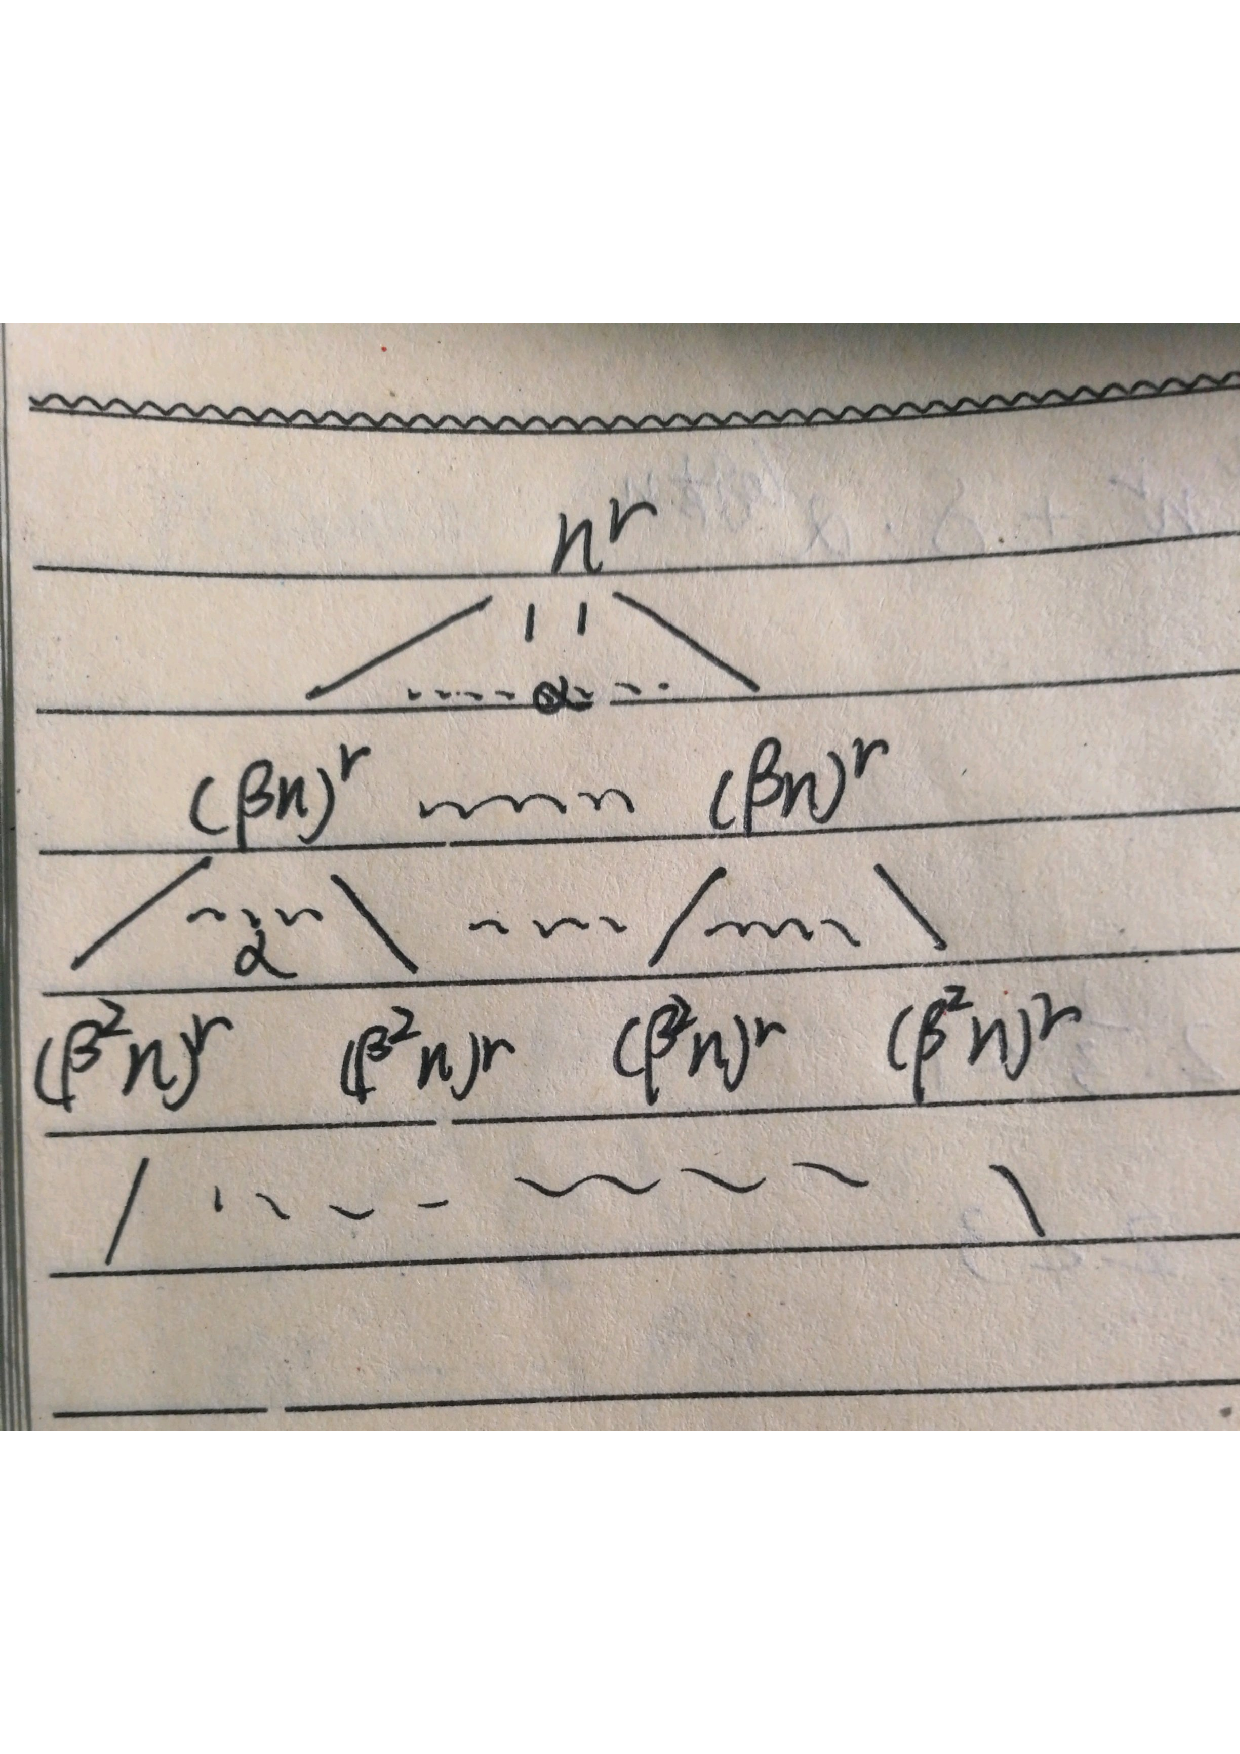
\includegraphics[scale=0.5]{images/p5.pdf}
    
    Sum of the second level: $\alpha (\beta n)^r$ \\
    Sum of the third level: $\alpha^2 (\beta^2 n)^r$ \\
    Sum of the fourth level: $\alpha^3 (\beta^3 n)^r$ \\
    Sum of the k-th level: $\alpha^k (\beta^k n)^r$
    
    Since $\beta$ < 1, we know there will be $log_\frac{1}{\beta} n$ levels and on the k-th level, there are $\alpha^k$ nodes, there will be $\alpha^{log_\frac{1}{\beta} n}$ nodes.
    
    T(n) = $n^r$ + $\alpha (\beta n)^r$  + $\alpha^2 (\beta^2 n)^r$ + ... + $\alpha^{log_\frac{1}{\beta} n -1} (\beta^{log_\frac{1}{\beta} n -1} n)^r$ = $\sum_{k=0}^{log_\frac{1}{\beta} n -1} (\alpha \beta^r)^k n^r$ + $\delta \alpha^{log_\frac{1}{\beta} n}$
    
    Since it is a geometric series, $\sum_{k=0}^{log_\frac{1}{\beta} n -1} (\alpha \beta^r)^k n^r$ = $\frac{n^{log(\alpha \beta^r) - 1}}{\alpha \beta^r -1} n^r$  
    
    Therefore, T(n) = $\frac{n^{log_\frac{1}{\beta}(\alpha \beta^r) - 1}}{\alpha \beta^r -1} n^r$  + $\delta n^{log_\frac{1}{\beta} \alpha}$. Hence, T(n) = O($n^{log_\frac{1}{\beta}(\alpha \beta^r) + r}$)
    
    \item If $\alpha \beta ^r$ < 1, we know the following
    \begin{enumerate}
        \item $\alpha < (\frac{1}{\beta})^r$
        \item T(n) = $\frac{1 - n^{log_\frac{1}{\beta}(\alpha \beta^r)}}{1 - \alpha \beta^r} n^r$  + $\delta n^{log_\frac{1}{\beta} \alpha}$.
    \end{enumerate}
    Hence, T(n) $\le$ $\frac{1 - 0}{1 - \alpha \beta^r} n^r$  + $\delta n^r$ $\le$ O($n^r$).
    
    \item If $\alpha \beta ^r$ = 1, we know the following
    \begin{enumerate}
        \item $\alpha = (\frac{1}{\beta})^r$
        \item T(n) = $n^r$ + $\alpha (\beta n)^r$  + $\alpha^2 (\beta^2 n)^r$ + ... + $\alpha^{log_\frac{1}{\beta} n -1} (\beta^{log_\frac{1}{\beta} n -1} n)^r$ = $\sum_{k=0}^{log_\frac{1}{\beta} n -1} (\alpha \beta^r)^k n^r$ + $\delta \alpha^{log_\frac{1}{\beta} n}$ = $\sum_{k=0}^{log_\frac{1}{\beta} n -1} n^r$ + $\delta n^{log_\frac{1}{\beta} \alpha}$ $\le$ O($n^r log n$)
    \end{enumerate}
    
\end{enumerate}
\end{numedquestion}

\pagebreak
\begin{numedquestion}
\begin{enumerate}[(a)]
    \item We can modify the Dijkstra's algorithm a bit. Beside its distance from source, we also record, for each vertex, the number of edges needed to reach it from the source. In the end, we can simply find the smallest distance \\
    \textbf{Algorithm:} Below is the pseudo-code 
    \begin{lstlisting}[mathescape=true]
    DijKEdges(G,K):
        H <- new heap
        numOfEdges <- a list records how many edges needed to 
                      reach a vertex from s 
        H.insert(s,0)
        numOfEdges(s) = 0
        for all v $\ne$ s:
            H.insert(s,$\infty$)
        
        while H not empty:
            (v,p) <- H.removeMin()
            dist(v) = p
            for each neighbour u of v:
                if u is unlabeled in H:
                    H.decrease(u,dist(v)+weight(v->u))
                    numOfEdges(u) = numOfEdges(v) + 1
        
        Iterate numOfEdges to find the smallest distance with the length of K
    \end{lstlisting}
    
    \textbf{Analysis:} Dijkstra takes O(E + VlogV) and the iteration in the end takes O(V) time, hence the algorithm takes O(E + VlogV) in total
    
    \textbf{Correctness:} Dijkstra will gives us the shortest distance between each vertex and the source. We set the number of edges of the vertex we are updating distance of to be 1 + the number of edges of the previous vertex, this means by taking this edge, we can reach this vertex with the distance we are updating to. This correctly records the number of edges needed to reach this vertex from the source with the recorded distance 
    
    \item We can modify the BellmanFord's algorithm a bit. Beside its distance from source, we also record, for each vertex, the number of edges needed to reach it from the source. In the end, we can simply find the smallest distance \\
    
    \textbf{Algorithm:}
    \begin{lstlisting}
    BFKEdges(G,K):
        dist(s) <- 0
        numOfEdges <- a list records how many edges needed to 
                      reach a vertex from s
        numOfEdges(s) <- 0
        for every vertex v $\ne$ s:
            dist(v) <- $\infty$
        
        for i <- 1 to v <- 1:
            for every edge u->v:
                if dist(v) > dist(u) + weight(u->v):
                    dist(v) = dist(u) + weight(u->v)
                    numOfEdges(v) <- numOfEdges(u) + 1
        Iterate numOfEdges to find the smallest distance with the length of K
    \end{lstlisting}
    
    \textbf{Analysis:} BellmanFord takes O(VE) and the iteration in the end takes O(V) time, hence the algorithm takes O(VE) in total 
    
    \textbf{Correctness:} BellmanFord will gives us the shortest distance between each vertex and the source, with the presence of negative edges. We set the number of edges of the vertex we are updating distance of to be 1 + the number of edges of the previous vertex, this means by taking this edge, we can reach this vertex with the distance we are updating to. This correctly records the number of edges needed to reach this vertex from the source with the recorded distance 
    
    \item We can run the algorithm in question 1 for each vertex and traverse numOfEdges in the end to find the global minimal k-edge walk. It takes O(VE + V*VlogV)
    
    \item We can modify the FloydWarshall's algorithm a bit. Beside the distance, we also record, for each vertex, the number of edges needed to reach it. In the end, we can simply find the smallest distance \\
    
    \textbf{Algorithm:}
    \begin{lstlisting}
    FWKEdges(G,K):
        numOfEdges <- a list records how many edges are in between
                      two vertices
                      
        for all vertices u:
            for all vertices v: 
                dist(u,v) <- w(u->v)
                numOfEdges(u,v) = 1
        
        for all vertices r:
            for all vertices u:
                for all vertices v:
                    if dist(u,v) > dist(u,r) + dist(r,v):
                        dist(u,v) = dist(u,r) + dist(r,v)
                        numOfEdges(u,v) = numOfEdges(u,r) + numOfEdges(r,v)
                        
       Iterate numOfEdges to find the smallest distance with the length of K 
    \end{lstlisting}
    \textbf{Analysis:} FloydWarshall takes O($V^3$) and the iteration in the end takes O(V) time, hence the algorithm takes O($V^3$) in total 
    
    \textbf{Correctness}: FloydWarshall will gives us the shortest distance between each pair of vertices, with the presence of negative edges. We set the number of edges on the path we are updating distance of to be the sum of the number of edges along the path via the middle vertex, this means to reach this vertex with the distance we are updating to, we need to go through the middle vertex. This correctly records the number of edges on the path from one vertex to another. 
\end{enumerate}
\end{numedquestion}

\pagebreak
\begin{numedquestion}
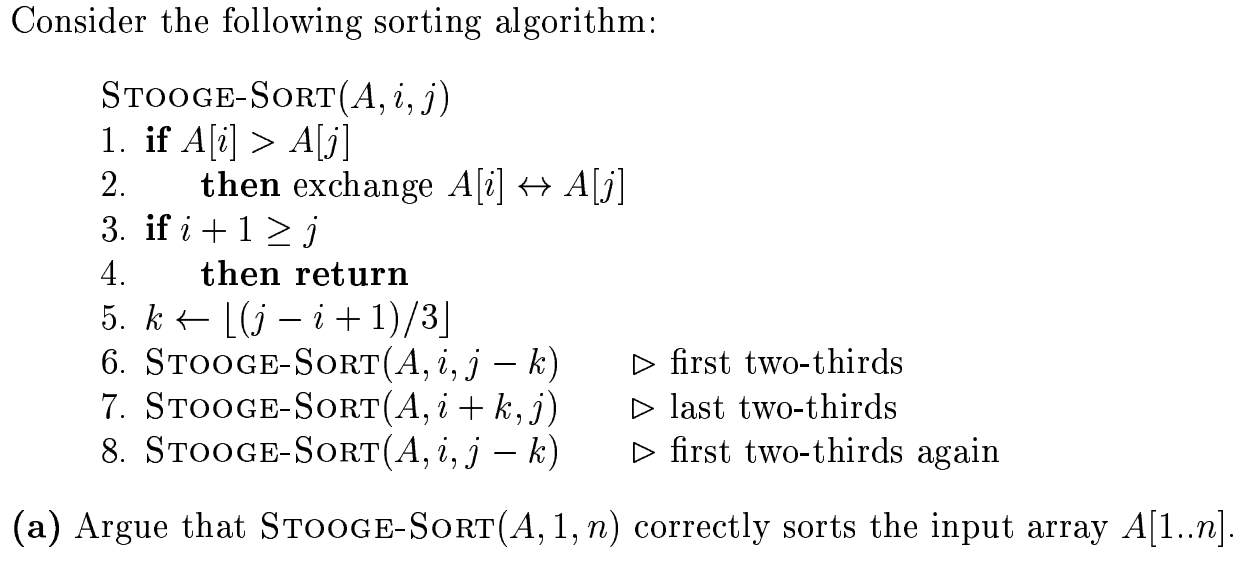
\includegraphics[scale=0.5]{images/q7a.PNG}\\
We prove by induction\\
\textbf{Base Case:} The algorithm clearly works for single-element and two-elements arrays \\ 
\textbf{Inductive Hypothesis}: The algorithm works for all arrays shorter than A[i,j]\\
\textbf{Induction step:} 
\begin{enumerate}
    \item After the execution of line 6, we know A[i,j-k] is sorted, due to the hypothesis. Therefore, each element in A[i+k,j-k] is no smaller than each element in A[i,i+k-1]. 
    
    \item After the execution of line 7, we know A[i+k,j] is sorted due to the hypothesis. Therefore, each element in A[j-k+1,j] is no smaller than A[i+k,j-k]
    
    Combining the above two results, we know each element in A[j-k+1,j] is no smaller than each element in A[i,i+k-1]. Hence, each element in A[j-k+1,j] is no smaller than each element in A[i,j-k]. 
    
    \item After the exeuction of line 8, we know A[i,j-k] is sorted due to the hypothesis. Since A[j-k+1,j] is also sorted as a result of line 7, we know A[i,j] is sorted. 
\end{enumerate}

(b) State the recurrance for worst case and the lower bound \\
T(n) = 3T($\frac{2n}{3}$) + O(1)\\

\end{numedquestion}

\pagebreak
\begin{numedquestion}
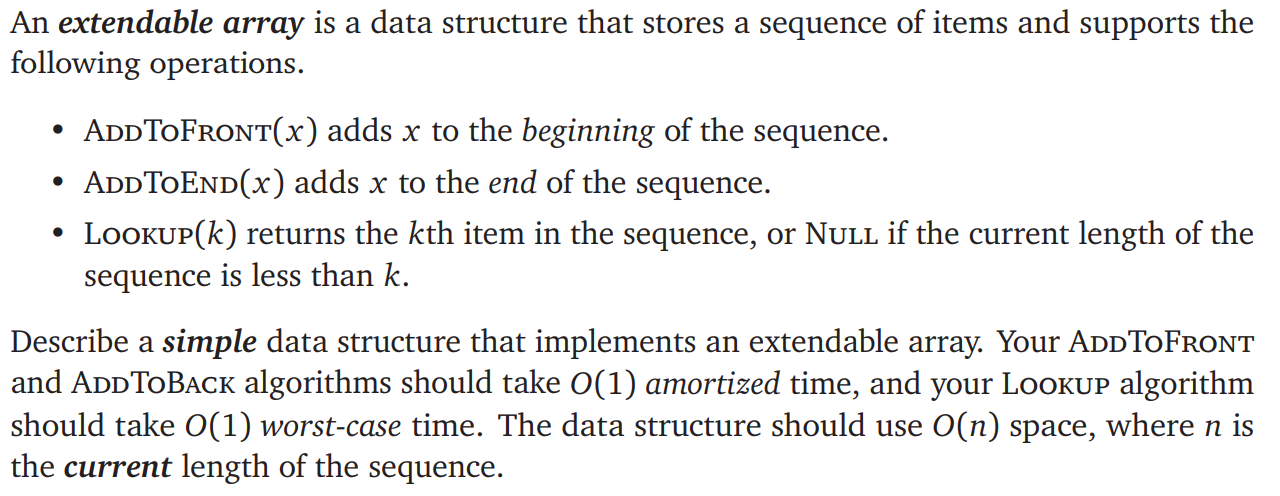
\includegraphics[scale=0.5]{images/q8.PNG}
\textbf{Data Structure:} We can use two arrays both of size n to achieve this, one array is for AddToFront and another for AddToEnd. We also keep two counters counting how many items are in each array, call them c1 and c2. For both arrays, we add an item as usual, which is AddToEnd. We do two special things to achieve our goal. 
\begin{enumerate}
    \item If one of the array is full, we expand the array by twice the size
    \item When looking up an item, we do the following
    \begin{enumerate}
        \item We first check if k > c1 + c2. If it is, we return null
        \item Then we check if k < c1. Since c1 holds the number of items in the array AddToFront, which stores the foremost items, if k > c1, we know the item is in AddToEnd array. Since we add a new item to the end of the array, the foremost item is actually at the back of the array. Hence, the index of the item we are really looking for is c1-k. 
        \item If k > c1, then we know we are looking for an item in AddToFront array. Since the first item in this array actually starts at index c1+1 in the sequence, the index of the item is actually k-c1.
    \end{enumerate} 
\end{enumerate}

\textbf{Analysis:} We look at the time complexities and the space complexity
\begin{enumerate}
    \item Space: We keep two arrays of size n and two counters, clearly the space is O(n)
    \item AddToFront Time: We use the accounting method. Supposed we have added n items to AddToFront, we need to expand the array by twice. We do this by allocating a new array twice the size of the current one, then we pop items in the current array and perform a AddToFront operation on the item to the new allocated array. Then for a single AddToFront operation, we assign \$2, one for add and one to pop it out later. Hence, the amortized time for a single AddToFront operation is O(1)
    \item AddToEnd Time: Same logic as above
    \item Look Up Time: Since look up would simply be index accessing, the worst time is O(1)
\end{enumerate}
\end{numedquestion}

\pagebreak
\begin{numedquestion}
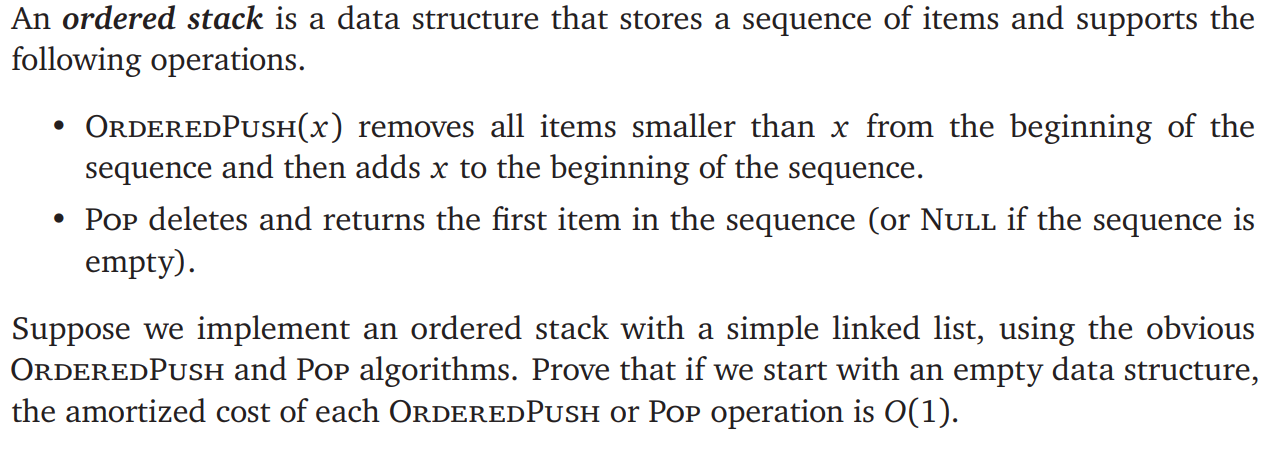
\includegraphics[scale=0.5]{images/q9.PNG}
\begin{enumerate}
    \item We first show for Pop. Since we just remove the head of the linked list, this takes constant time. It is independent of the size of the stack, so it is O(1) time worst case, so obviously also O(1) amortized
    \item We then show for OrderedPush. We use the accounting method. For each OrderedPush, we charge x \$3
    \begin{enumerate}
        \item One is for comparing with the top of the stack. Since the stack is ordered and the top is the smallest, if the top is already larger than x, no more comparison is needed
        \item One is to add x to the stack
        \item Another is saved for later. At a later time when x is already on the stack and is compared with a new item, there can be two cases. If x is larger than the new item, the new item has already paid for this, as mentioned above. If x is smaller than the new item, x use this dollar to delete itself.  
    \end{enumerate}
    Therefore, the amortized cost for push is O(1)
\end{enumerate}
\end{numedquestion}

\pagebreak
\begin{numedquestion}
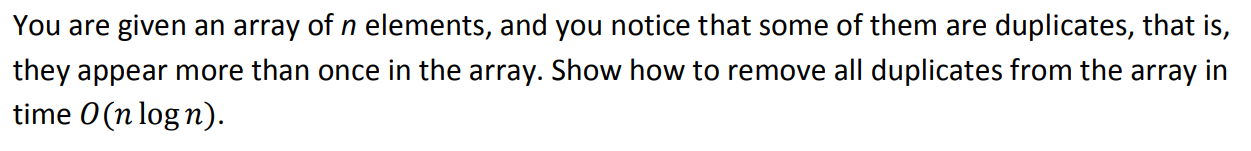
\includegraphics[scale=0.5]{images/q10.PNG}
We do a mergesort on the array, which cost O(nlogn), then we simply traverse the sorted array to delete duplicates, which cost O(n). Hence, the algorithm takes O(nlogn) in total 
\end{numedquestion}

\pagebreak
\begin{numedquestion}
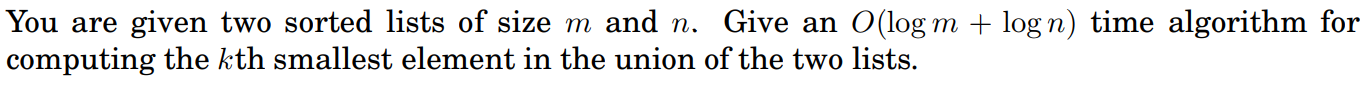
\includegraphics[scale=0.5]{images/q11.PNG}
We do something like binary search on the two arrays. If we think on the perspective of a merged array, the first half of this array will be first halves of both arrays. Therefore, the new mid = mid1 + mid2. Hence, we have the following scenarios
\begin{enumerate}
    \item mid1 + mid2 < k. This means the kth element is at the second half of the merged array. There could be two sub scenarios
    \begin{enumerate}
        \item arr1[mid1] > arr2[mid2]. This means mid1 is larger than all elements in the first half of arr2. Since k > mid1 + mid2, we know k cannot be on the first half of arr2, therefore, we don't need to search on the first half of arr2
        \item arr1[mid1] < arr2[mid2]. According to the same logic, we don't need to search on the first half of arr1
    \end{enumerate}
    
    \item mid1 + mid2 > k. This means the kth element is at the first half of the merged array. There could be two sub scenarios
    \begin{enumerate}
        \item arr1[mid1] > arr2[mid2]. This means mid1 is larger than all elements in the first half arr2. Since k is on the first half of the merged array, we don't need to search on the second half of arr2
        \item arr1[mid1] < arr2[mid2]. Same logic as above, we don't need to search on the second half of arr1
    \end{enumerate}
\end{enumerate}
Since we are basically performing binary searches on the two arrays, the time complexity is O(log m + log n)
\end{numedquestion}

\pagebreak
\begin{numedquestion}
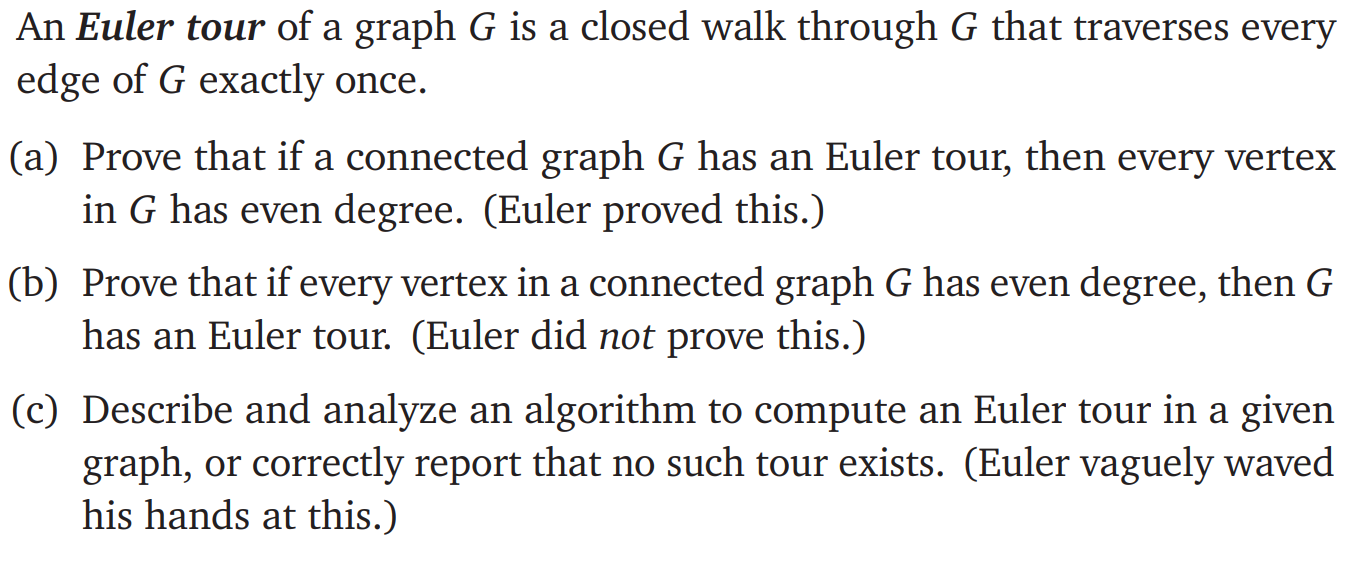
\includegraphics[scale=0.5]{images/q12.PNG}
\begin{enumerate} [(a)]
    \item Since Euler tour is a closed walk, we end the walk at the vertex where we started the walk. If we traverse every edge on the graph once, we must have visited every vertex on the graph as well. If we enter a vertex via one edge, we must be able to leave the vertex via another edge. Hence, every vertex has even number of edges
    
    \item If every vertex has even number of edges, then we are always able to enter the vertex through one edge and leave through another. If we revisit a vertex and there are still vertices we haven't visit, we know some edges are not used and we can always visit these vertices from some vertices we have visited, using some unused edges, since the graph is connected. After we visited these previously not-visited vertices, we know we can get back to vertices that were previously visited using some previously unused edges. Hence we can end at the vertex where we started the walk by using all the edges once. 
    
    \item We first look at if every vertex has even number of edges. If we find a vertex that doesn't have even number of edges, according to (a), we know the graph doesn't contain a Euler tour. 
    We can use the Hierholzer’s Algorithm. The gist of this algorithm is we start at a random vertex and follow a trail of edges from that vertex until returning to v. It is not possible to get stuck at any vertex other than v, because indegree and outdegree of every vertex must be same, when the trail enters another vertex w there must be an unused edge leaving w.The idea is to keep following unused edges and removing them until we get stuck. Once we get stuck, we back-track to the nearest vertex in our current path that has unused edges, and we repeat the process until all the edges have been used. We can use another container to maintain the final path. Since we visit each edge exactly once, the time is O(E).
\end{enumerate}
\end{numedquestion}
\pagebreak
\begin{numedquestion}
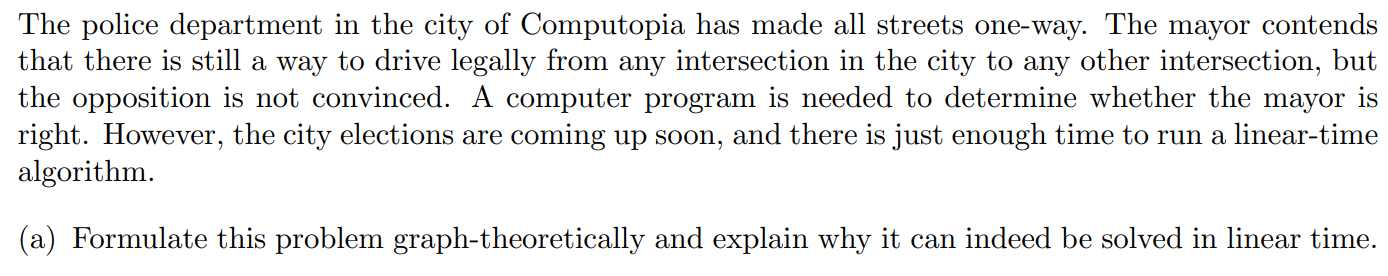
\includegraphics[scale=0.5]{images/q13.PNG}
This problem can be represented by a directed graph G = (V, E) where each intersection is a vertex
v and there is an edge between intersections (u, v) if there is a road that goes directly from u to
v. The criteria that there is a way to drive legally from any intersection to any other intersection
is true if, and only if, there is path from each vertex of G to every other vertex. This is true if,
and only if, the graph is Strongly connected, so this can be solved in linear time with DFS by
determining if the graph is a single strongly connected component.
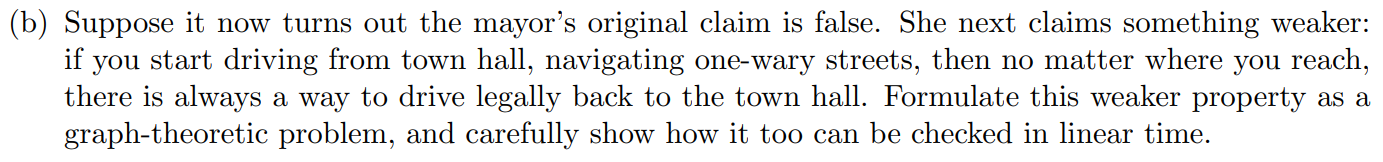
\includegraphics[scale=0.5]{images/q13b.PNG}
We use the same graph G as in the first part of the question and label the town hall s. This
property is true if, and only if, s cannot reach a vertex v, which can't reach back to s. Then there must be no path from s to a vertex outside of the connected component
of s. To determine if the graph has this property we can label each vertex with the number of its
connected component and then do a depth first search from s. If s can reach a vertex which is in
a different connected component then the new claim is false.
\end{numedquestion}

\pagebreak
\begin{numedquestion}
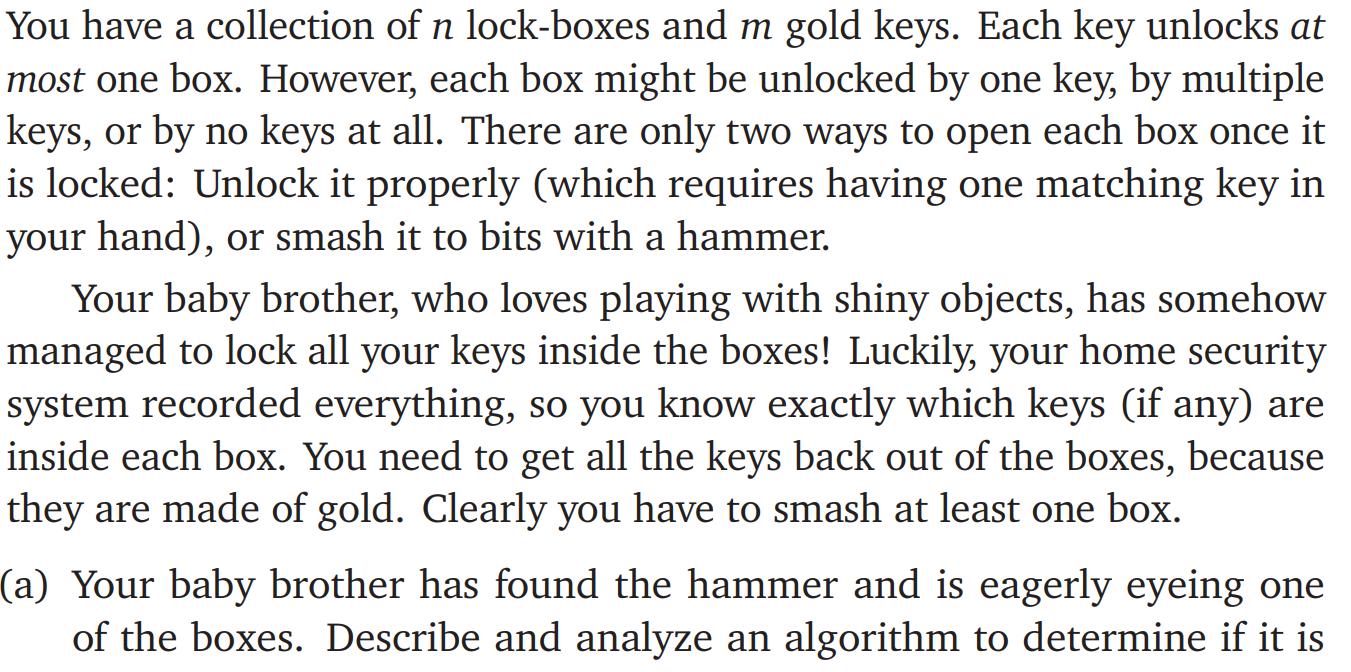
\includegraphics[scale=0.5]{images/q14.PNG}
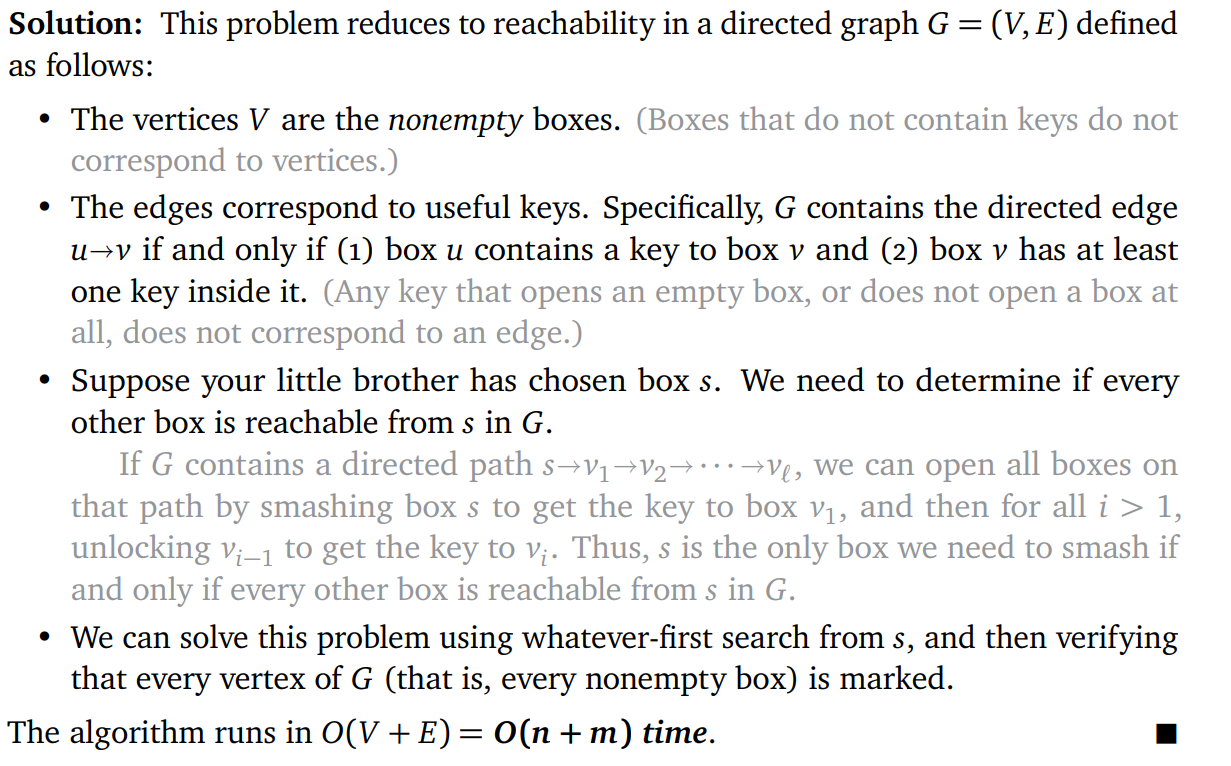
\includegraphics[scale=0.5]{images/q13aSol.PNG}

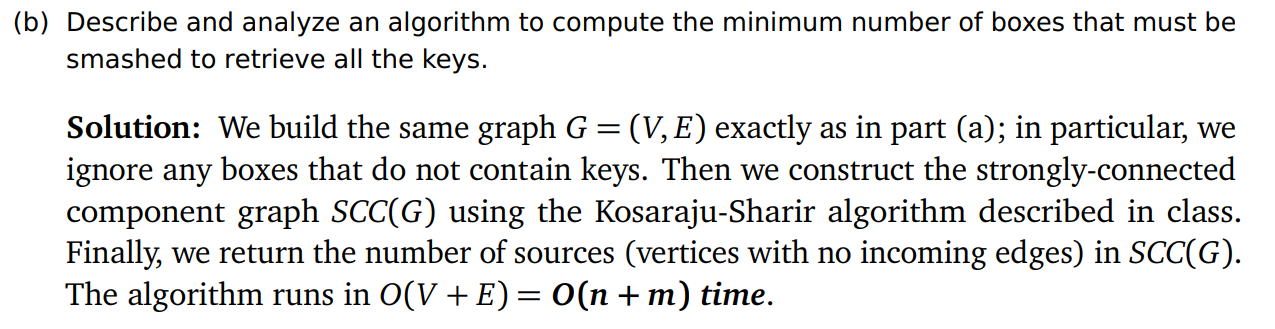
\includegraphics[scale=0.5]{images/q14b.PNG}
\end{numedquestion}

\pagebreak
\begin{numedquestion}
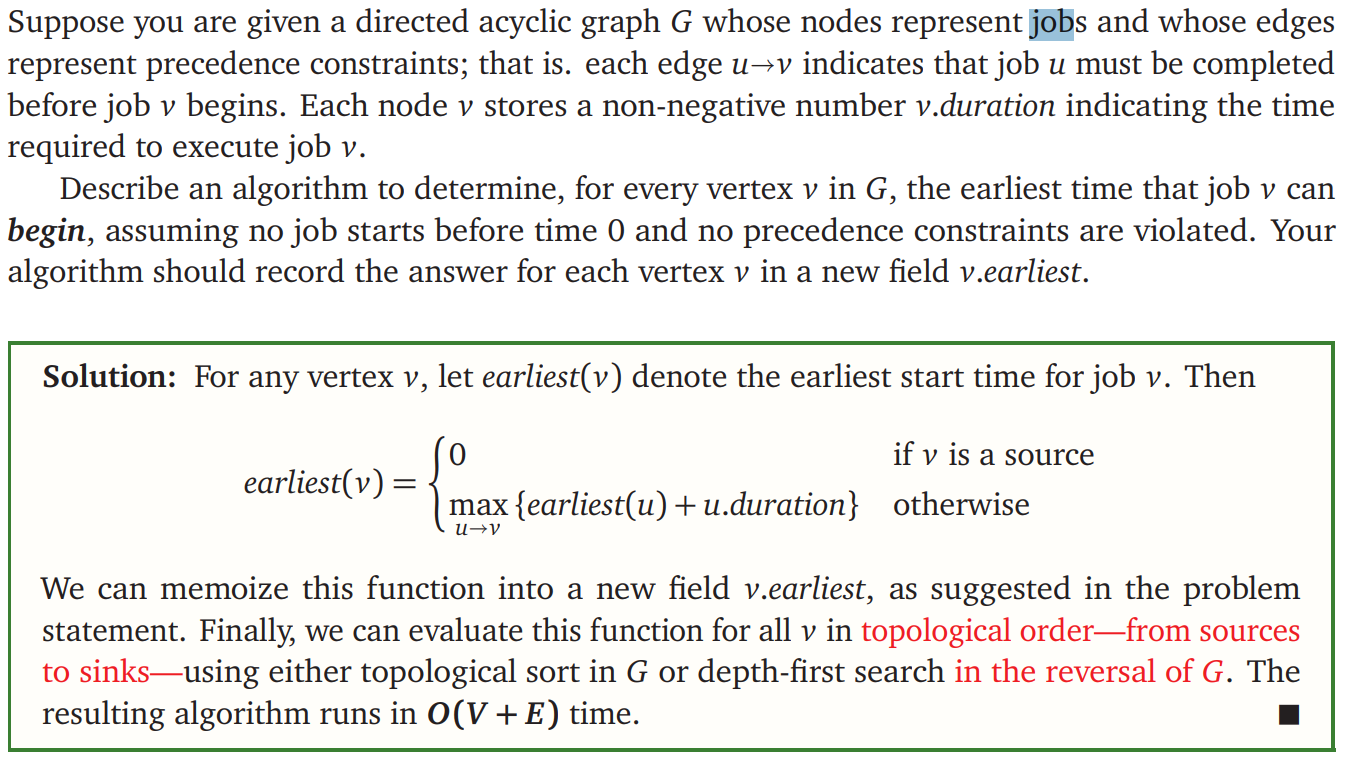
\includegraphics[scale=0.5]{images/q15.PNG}
\end{numedquestion}

\pagebreak
\begin{numedquestion}
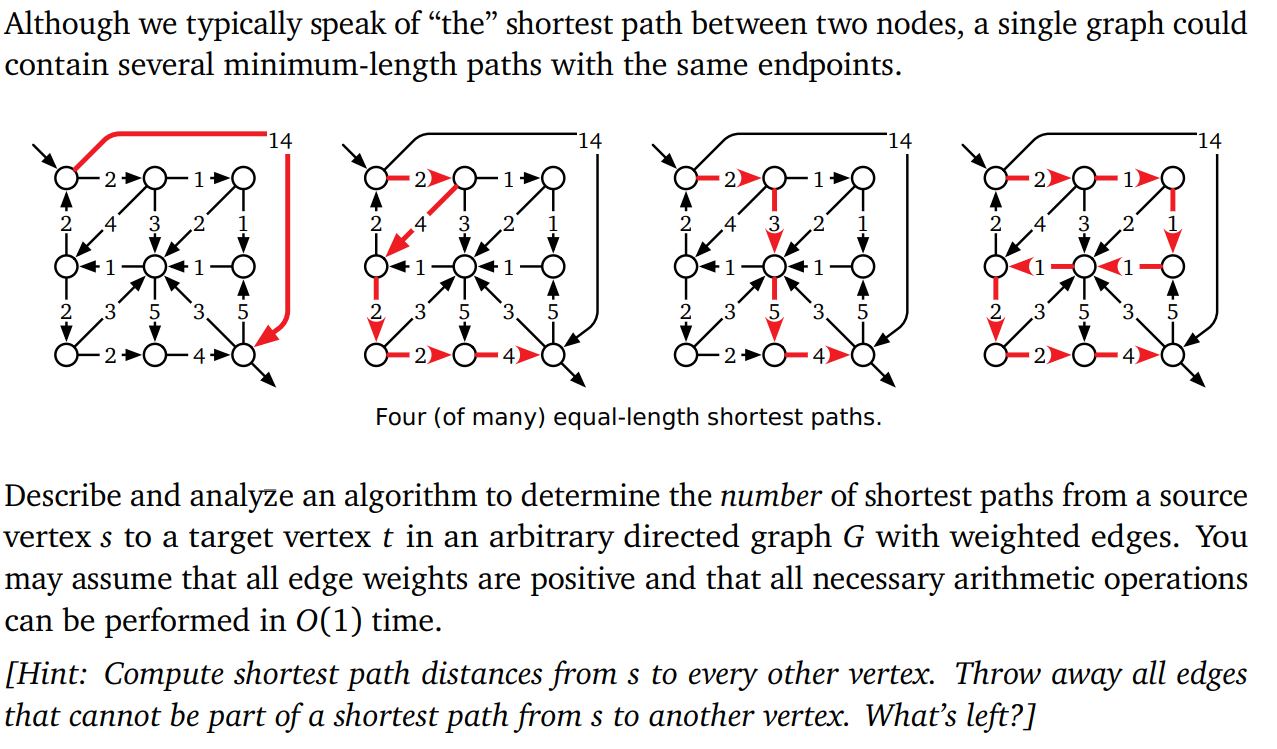
\includegraphics[scale=0.5]{images/q16.PNG}
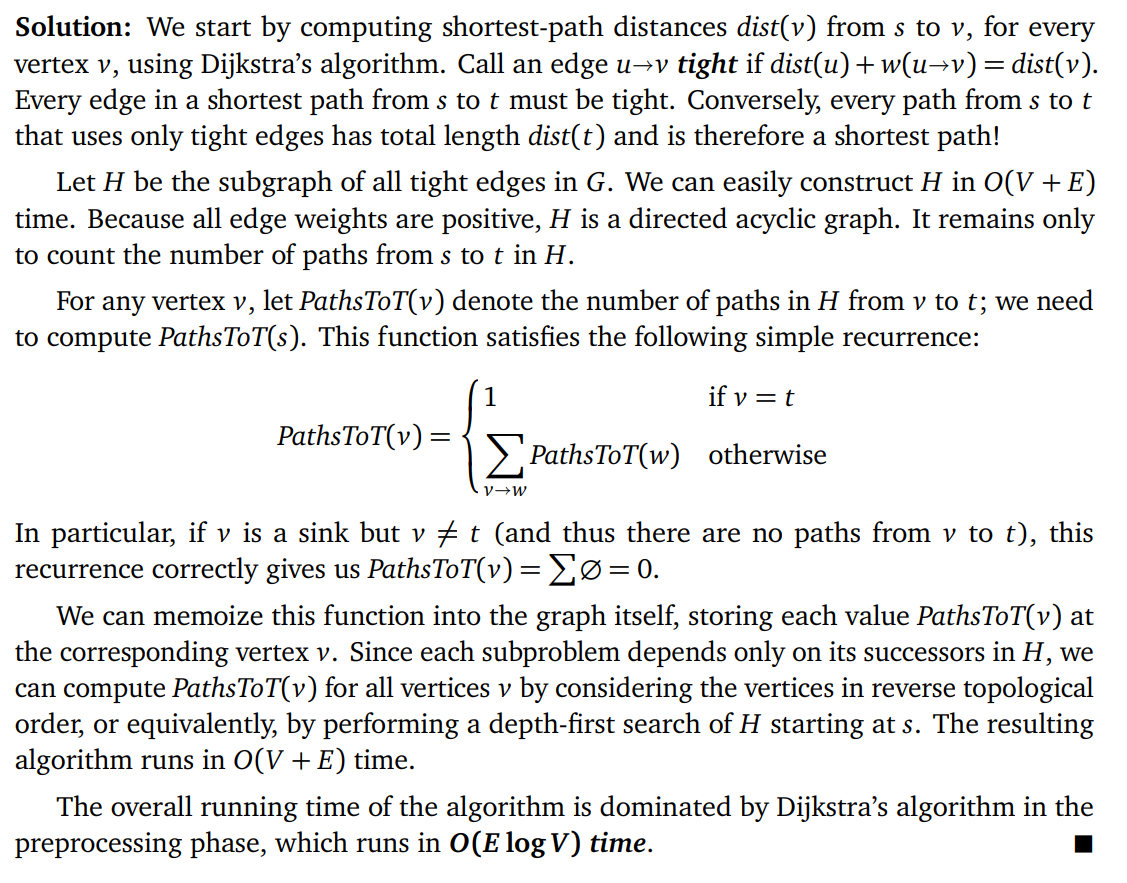
\includegraphics[scale=0.5]{images/q16sol.PNG}
\end{numedquestion}

\pagebreak
\begin{numedquestion}
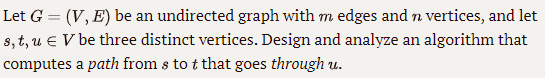
\includegraphics[scale=1]{images/q17.PNG} \\
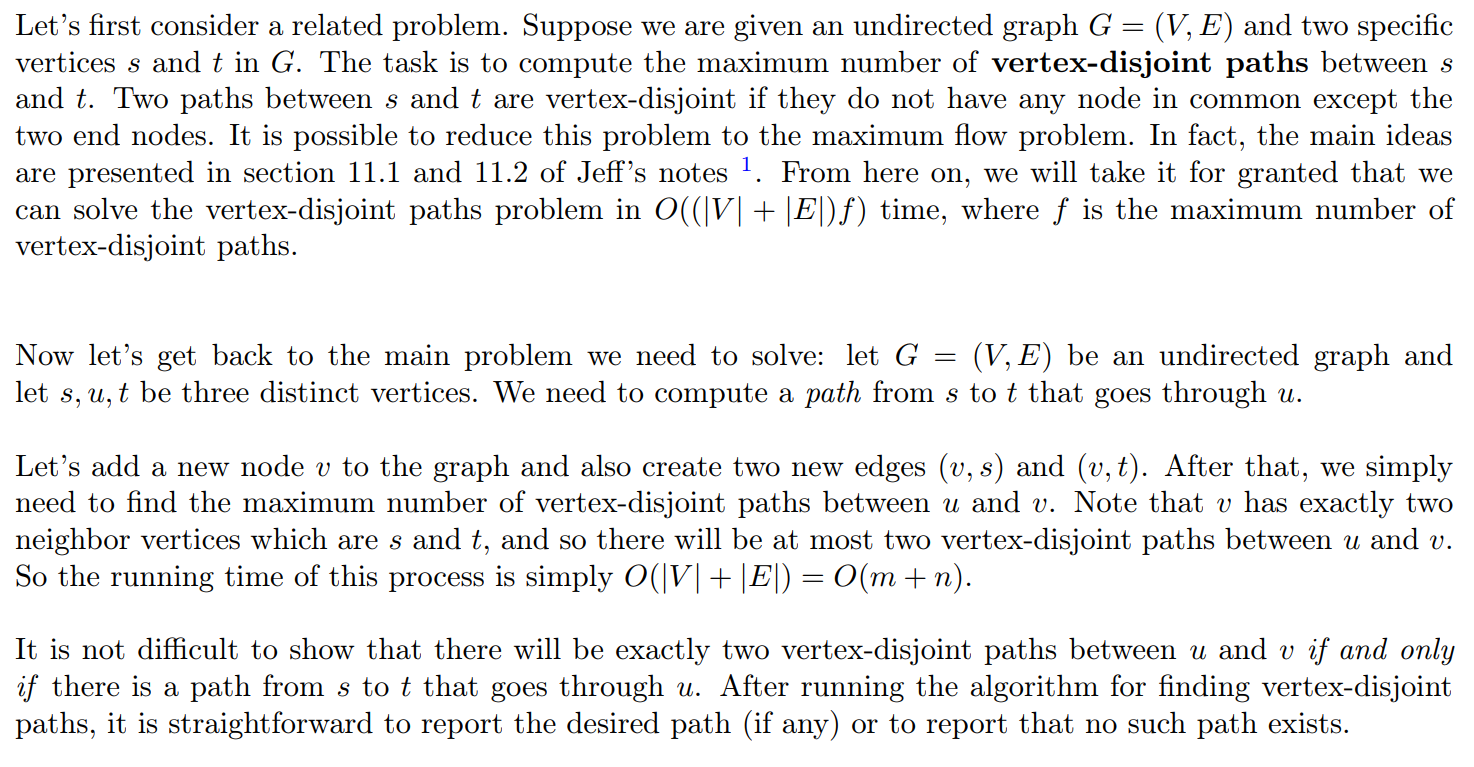
\includegraphics[scale=0.45]{images/q17sol.PNG}
\end{numedquestion}

\pagebreak
\begin{numedquestion}
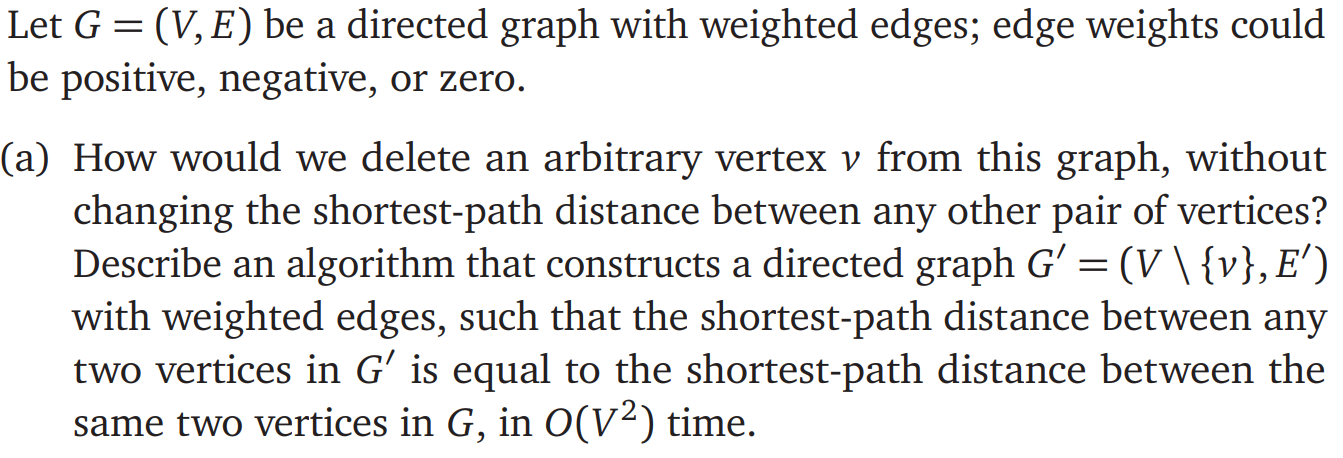
\includegraphics[scale=0.5]{images/q18.PNG}
This corresponds to the second inner loop of Floyd Warshall, with vertex r being the vertex being deleted. Here is the algorithm:\\
\begin{lstlisting}
for all neighbour u of v with an edge u->v:
    for all neighbour w of v with an edge v->w:
        if edge u->w doens't exist:
            add an edge u->w with weight w(u,v) + w(v,w)
        else:
            if w(u,w) > w(u,v) + w(v,w):
                set w(u,w) <- w(u,v) + w(v,w)
\end{lstlisting}
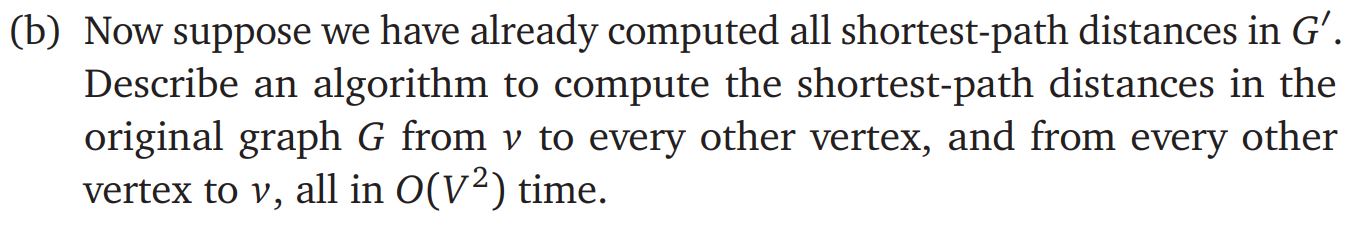
\includegraphics[scale=0.5]{images/q18b.PNG}
\begin{enumerate}
    \item From v to every other vertex
    \begin{lstlisting}
    for all vertex u other than v:
        if there is no edge v->u:
            for all neighbour w with an edge v->w:
                dist(v,u) <- w(v,w) + dist(w,u)
        else:
            dist(v,u) <- w(v,u)
    \end{lstlisting}
    
    \item From every other vertex to v
    \begin{lstlisting}
      for all vertex u other than v:
        if there is no edge u->v:
            for all neighbour w with an edge w->v:
                dist(u,v) <- w(w,v) + dist(u,w)
        else:
            dist(u,v) <- w(u,v)
    \end{lstlisting}
  
\end{enumerate}
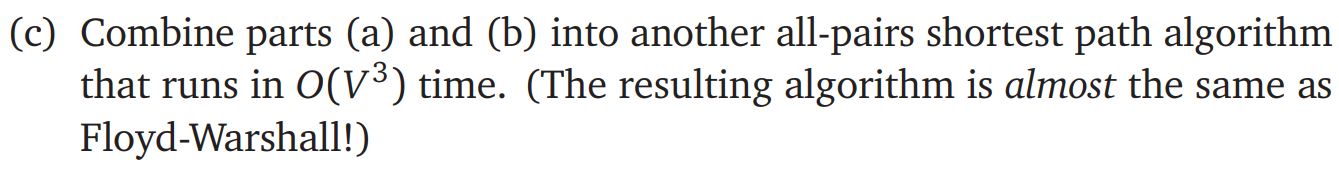
\includegraphics[scale=0.5]{images/q18c.PNG}
we treat (a) and (b) as blackboxes, call them bba and bbb
\begin{lstlisting}
    for all vertices u:
        for all vertices v:
            dist(u,v) <- w(u,v)
            
    for all vertex v:
        run bba to update dist
    
    for all vertex v:
        run bbb to incorporate v's dist information 
        
\end{lstlisting}
\end{numedquestion}

\pagebreak
\begin{numedquestion}
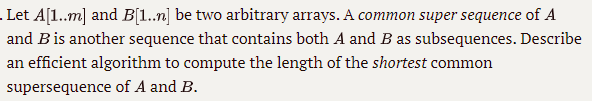
\includegraphics[scale=1]{images/q19.PNG} \\
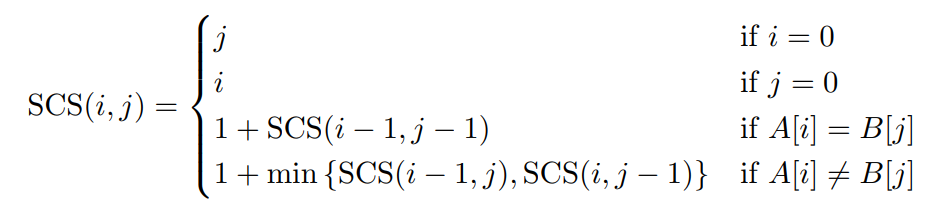
\includegraphics[scale=0.5]{images/q19sol.PNG}
\end{numedquestion}

\pagebreak
\begin{numedquestion}
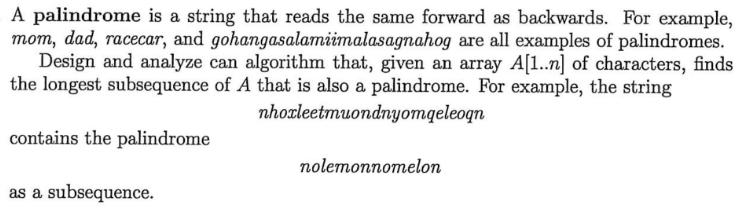
\includegraphics[scale=0.9]{images/q20.PNG}\\
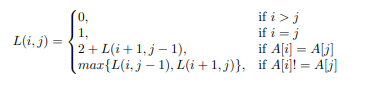
\includegraphics[scale=1]{images/q20sol.PNG}
\end{numedquestion}

\pagebreak
\begin{numedquestion}
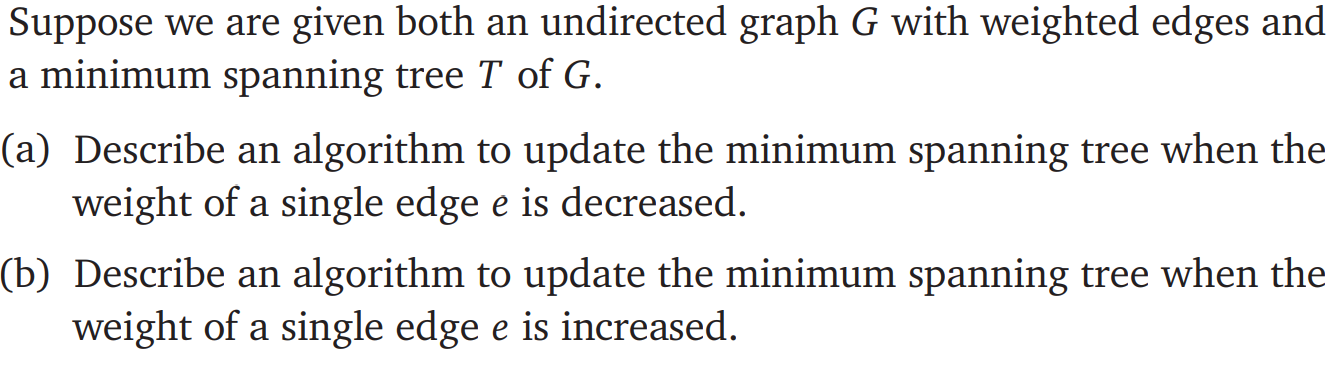
\includegraphics[scale=0.5]{images/q21.PNG}

\begin{enumerate}[(a)]
    \item there are two cases 
    \begin{enumerate}
        \item e $\in$ T\\
        In this case, T is still a MST
        \item e $\notin$ T\\
        Add e to T, this will create a cycle in T. We can find this cycle using DFS, which runs in O(V+E). Next, we can simply delete the maximum edge on the cycle to form a new MST. Since edges other than e and not on T will be heavier than edges on T and e, they can't be part of the new MST. Hence, the odd one out is simply in this cycle 
    \end{enumerate}
    
    \item There are two cases
    \begin{enumerate}
        \item e $\notin$ T\\
        In this case, T is still a MST
        
        \item e $\in$ T\\
        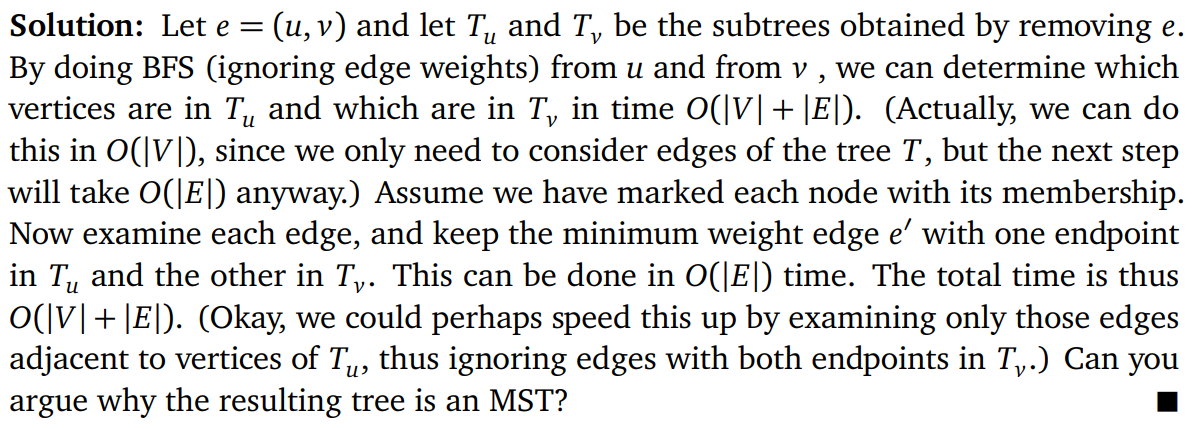
\includegraphics[scale = 0.5]{images/q21sol.PNG}
    \end{enumerate}
\end{enumerate}
\end{numedquestion}

\pagebreak
\begin{numedquestion}
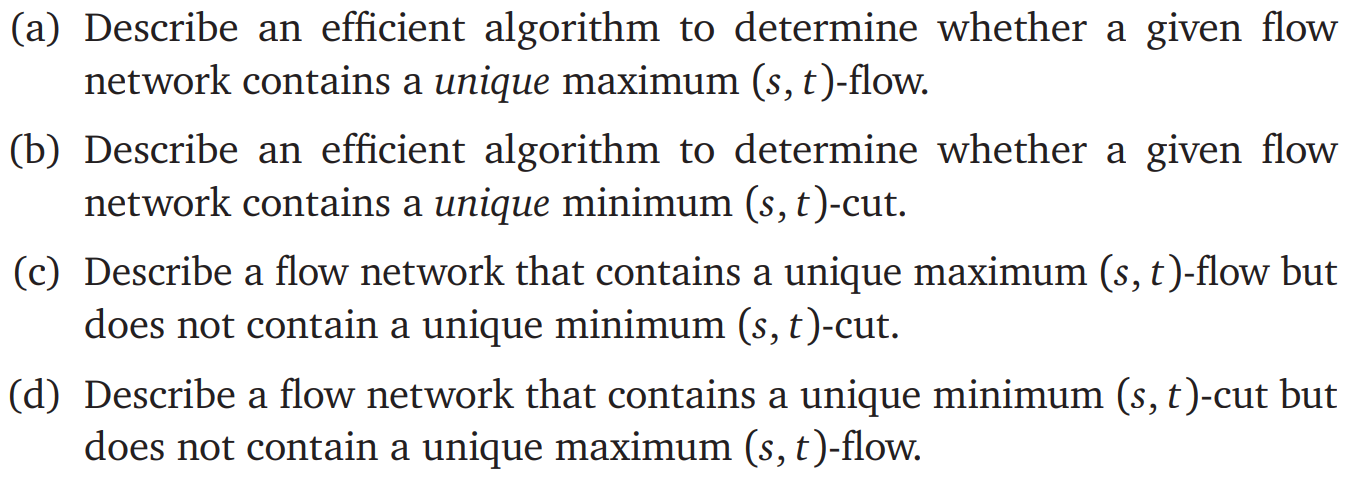
\includegraphics[scale=0.5]{images/q22.PNG}
\begin{enumerate}[(a)]
    \item Find a maximum flow. Then create m new flow networks: one for each edge in the maximum flow. In each new configuration, reduce the capacity of one of the edges to an amount just below its flow. Find the maximum flow on each of the new flow networks. If any of the new configurations generate the same maximum flow value as the original graph, then that new flow is also a maximum flow in the original graph. Hence, the original maximum flow is not unique.
    
    \item 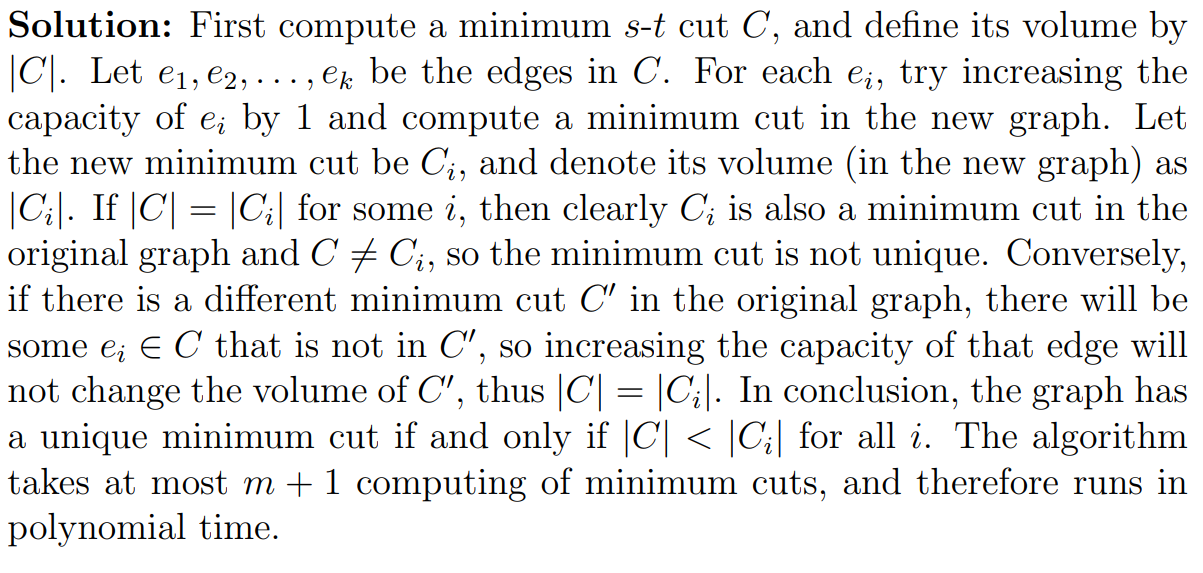
\includegraphics[scale=0.5]{images/q22bsol.PNG}
    
    \item A link-list like graph from s to t, where each edge has the same capacity 
    
    \item 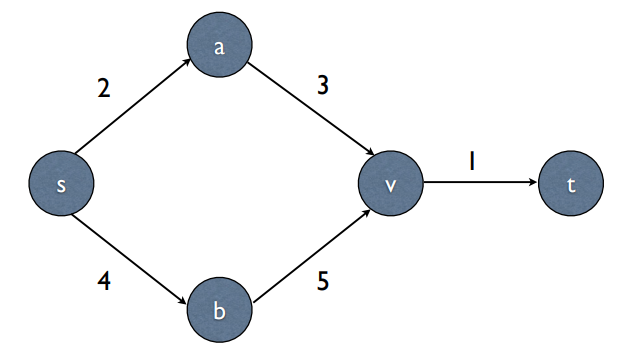
\includegraphics[scale=0.5]{images/q22dsol.PNG}
\end{enumerate}
\end{numedquestion}

\pagebreak
\begin{numedquestion}
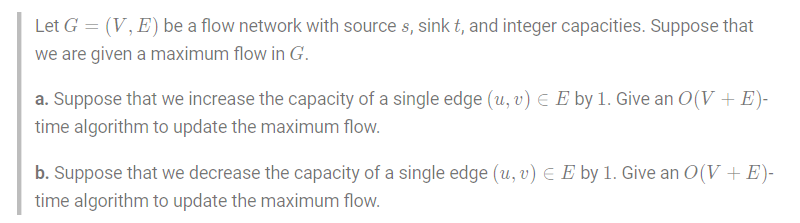
\includegraphics[scale=0.9]{images/q23.PNG}\\
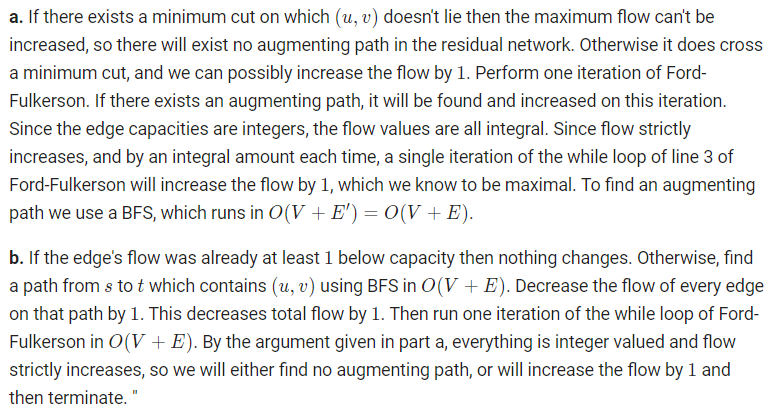
\includegraphics[scale=0.9]{images/q23sol.PNG}
\end{numedquestion}

\pagebreak
\begin{numedquestion}
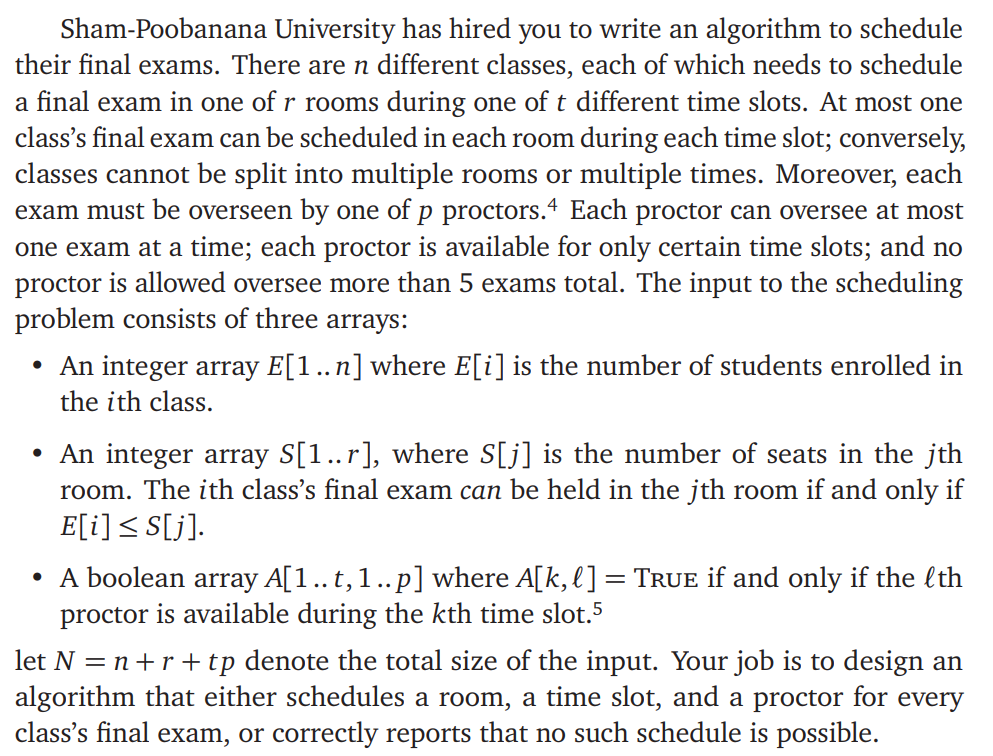
\includegraphics[scale=0.6]{images/q24.PNG}\\
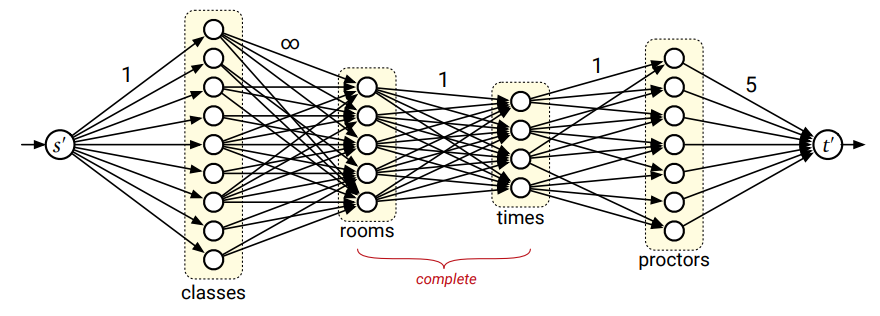
\includegraphics[scale=0.8]{images/q24Pic.PNG}\\
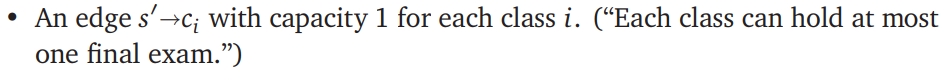
\includegraphics[scale=0.6]{images/q21Sol1.PNG}\\
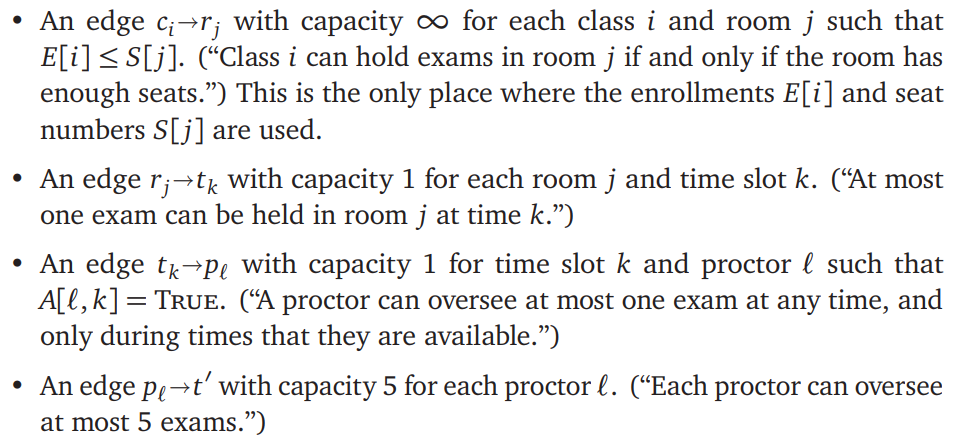
\includegraphics[scale=0.6]{images/q24sol2.PNG}\\
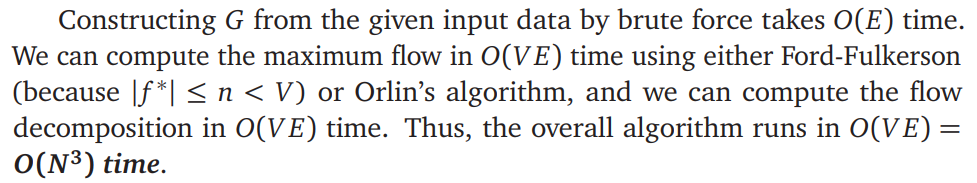
\includegraphics[scale=0.6]{images/q24anl.PNG}\\
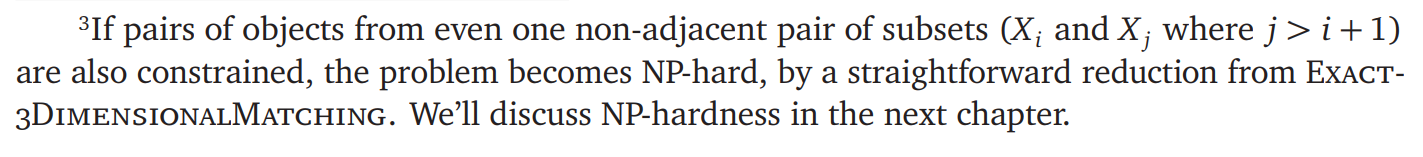
\includegraphics[scale=0.5]{images/q24Note.PNG}
\end{numedquestion}

\pagebreak
\begin{numedquestion}
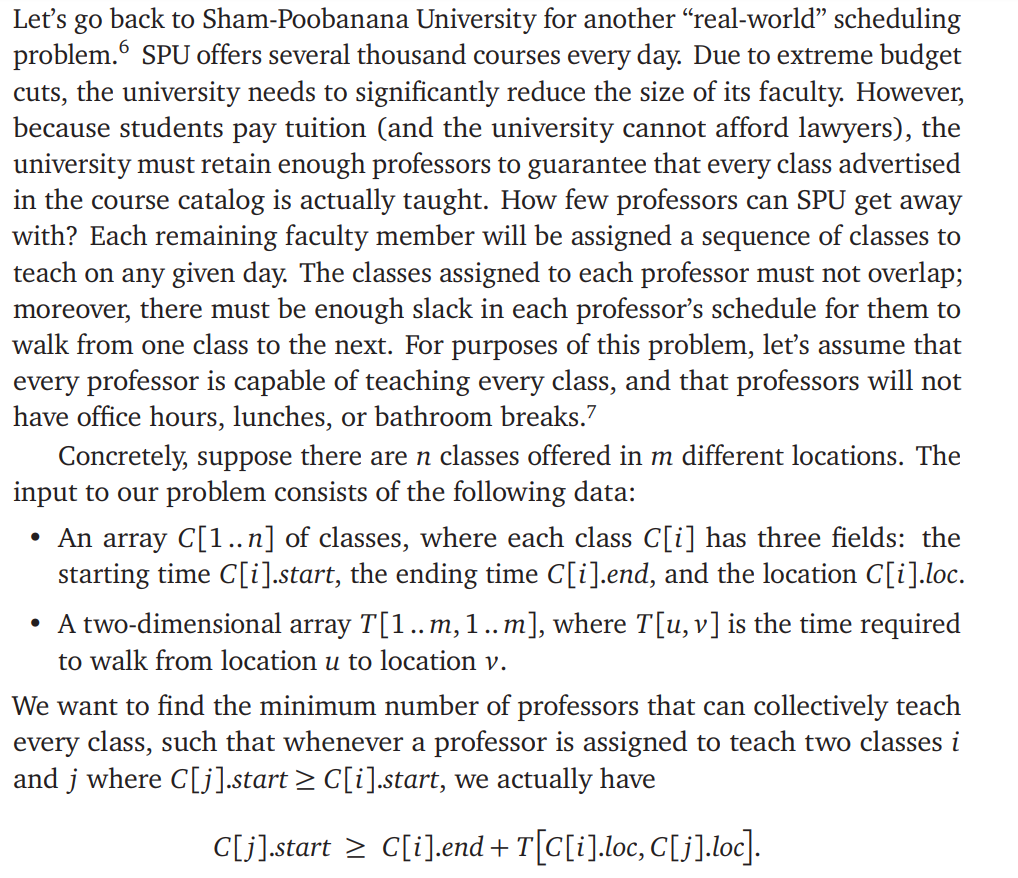
\includegraphics[scale=0.6]{images/q25.PNG}\\
We can solve this problem by reducing it to a disjoint-path cover problem as follows. We construct a dag G = (V, E) whose vertices are classes and whose edges represent pairs of classes that are scheduled far enough apart to be taught by the same professor. Specifically, a directed edge i -> j indicates that the same professor can teach class i and then class j. It is easy to construct this dag in O($n^2$) time by brute force. Then we find a disjoint-path cover of G using the matching algorithm described above; each directed path in G represents a legal class schedule for one professor. The entire algorithm runs in O($n^2$ + V E) = O($n^3$) time
\end{numedquestion}

\pagebreak
\begin{numedquestion}
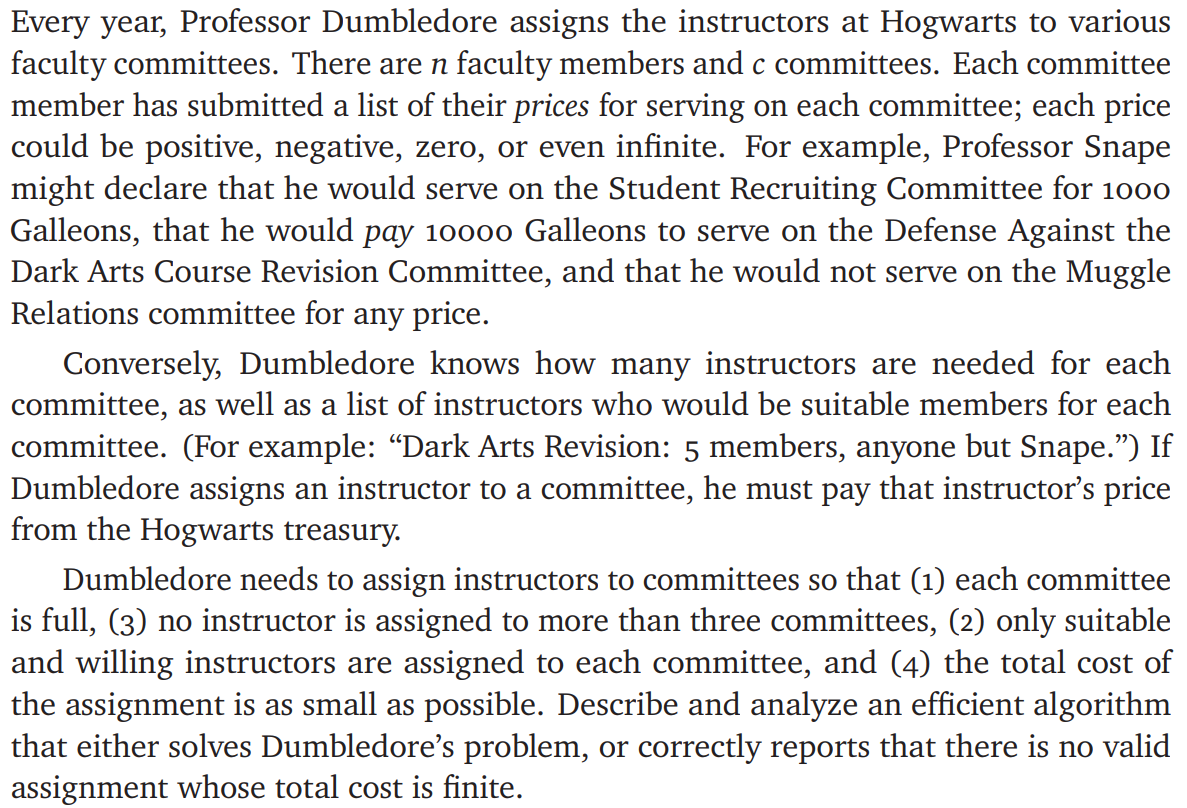
\includegraphics[scale=0.5]{images/q26.PNG} \\
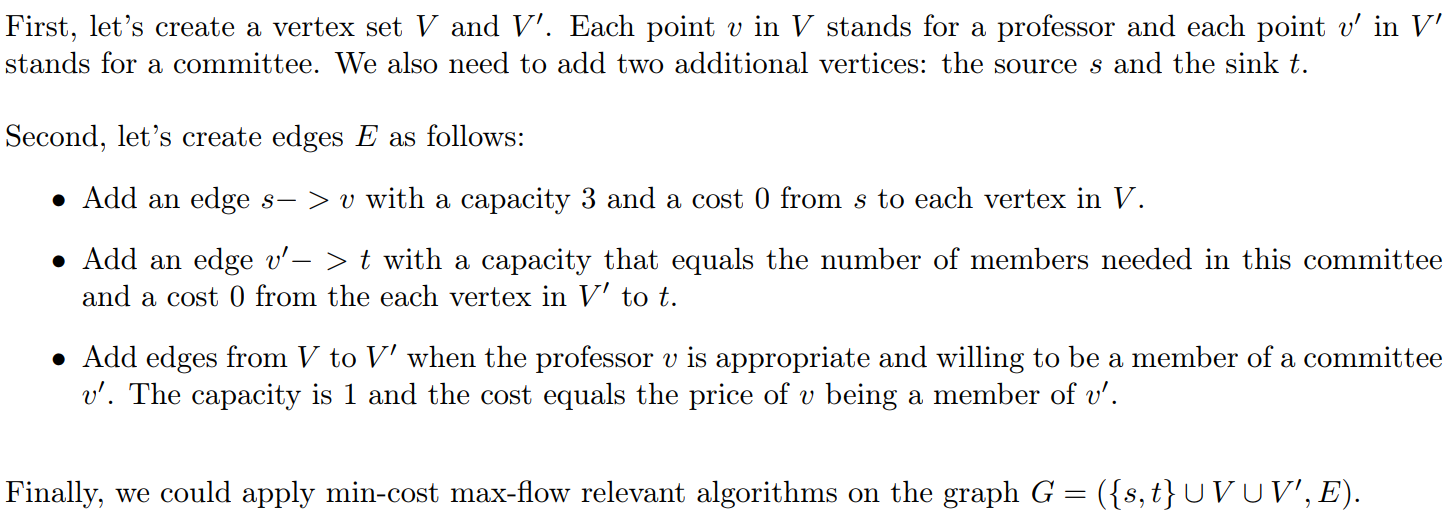
\includegraphics[scale=0.45]{images/q26sol.PNG}
\end{numedquestion}

\pagebreak
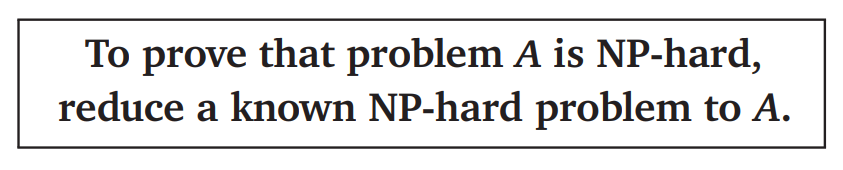
\includegraphics[scale=0.5]{images/NPRule.PNG}\\
\textbf{To reduce problem X to problem Y in polynomial time, we need to do three things}
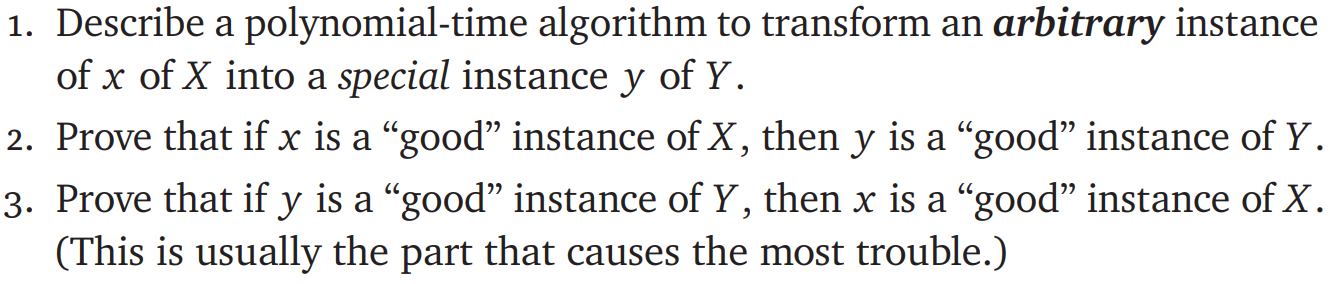
\includegraphics[scale=0.5]{images/NPSteps.PNG}

\pagebreak
\begin{numedquestion}
Prove SAT is NP-Hard \\

X = CircutSAT\\
Y = SAT\\

Step 1: \\
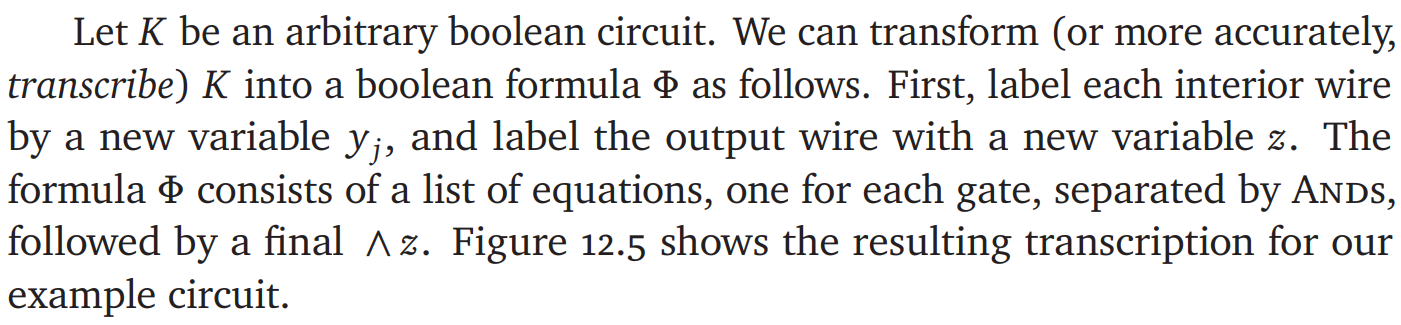
\includegraphics[scale=0.5]{images/q27.PNG} \\
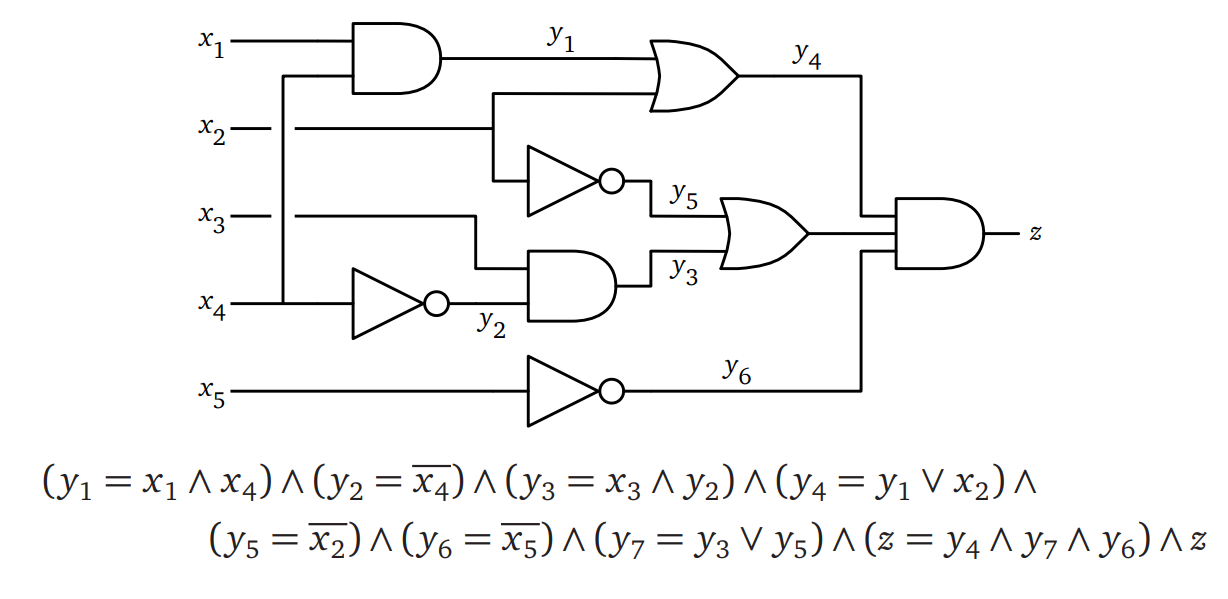
\includegraphics[scale=0.5]{images/q27Fig.PNG}\\

Step 2: Given a set of inputs that satisfy the circuit K, we can derive a satisfying assignment for the formula $\Phi$ by computing the output of every gate in K \\

Step 3: Given a satisfying assignment for the formula $\Phi$, we can obtain a satisfying input for the circuit by simply ignoring the internal wire variables yi and the output variable z.
\end{numedquestion}

\pagebreak
\begin{numedquestion}
Prove MaxClique is NP-hard \\

X = Max Independent Set\\
Y = Max Clique\\ 

Step1: \\
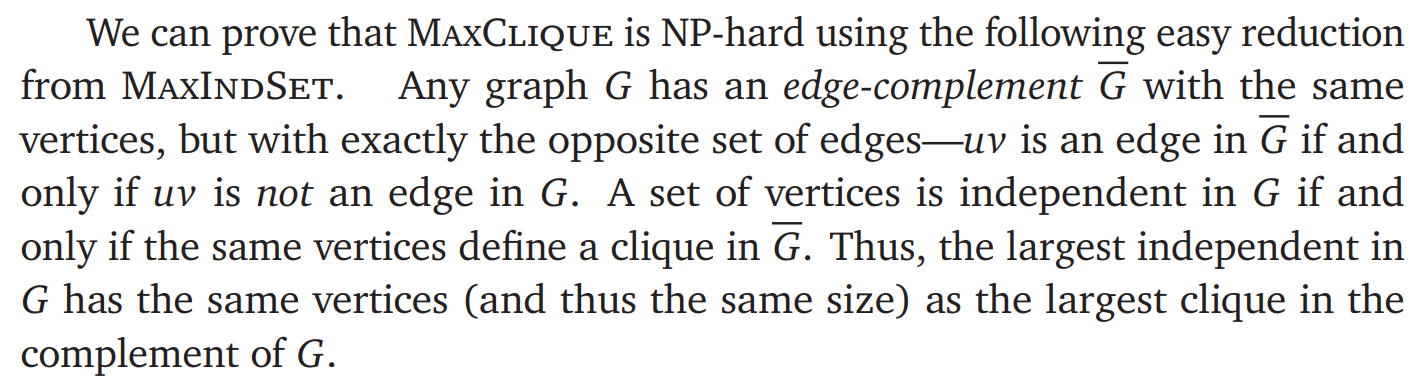
\includegraphics[scale=0.5]{images/q28.PNG}

Step2 and Step3 can be derived from the definition of max independent set and max clique 
\end{numedquestion}

\pagebreak
\begin{numedquestion}
Prove 3-Coloring is NP-hard \\

X = 3SAT\\
Y = 3-Coloring\\

Step1: \\
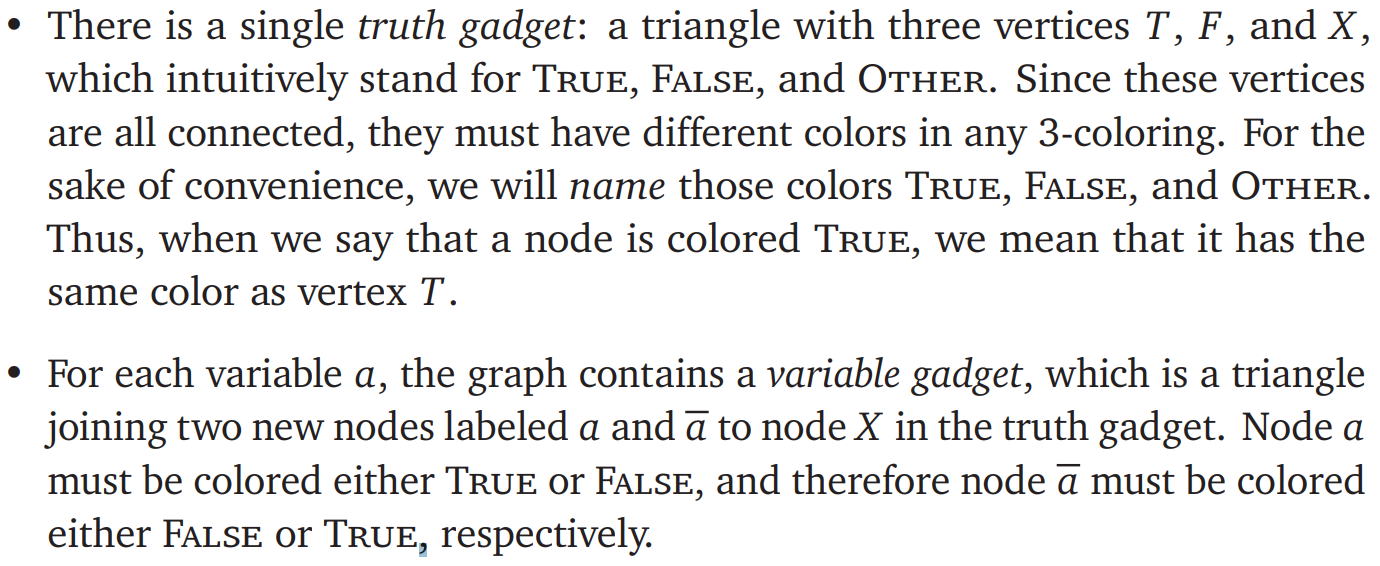
\includegraphics[scale=0.5]{images/q29a.PNG}
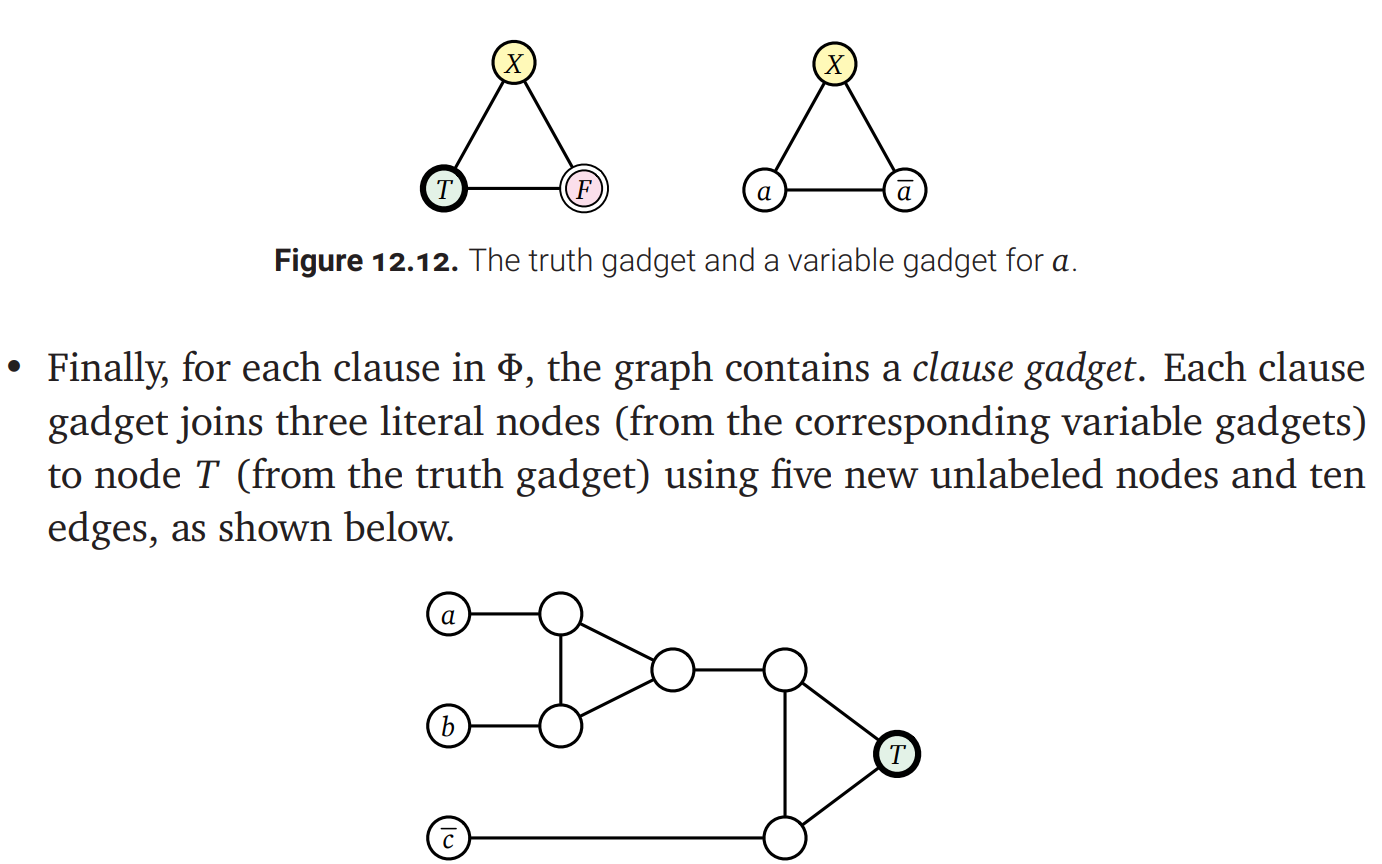
\includegraphics[scale=0.5]{images/q29b.PNG}

Step2: If the formula is satisfiable, then we can color the literal nodes according to any satisfying
assignment, and then (because each clause is satisfied) extend the coloring across every clause gadget. This is because the variable gadgets force each literal node to be colored either T or F; thus, in any valid -coloring of the clause gadget, at least one literal node is colored T\\

Step3: If the graph is 3-colorable, then we can extract a satisfying assignment from any 3-coloring—at least one of the three literal nodes in every clause gadget is colored T.
\end{numedquestion}

\pagebreak
\begin{numedquestion}
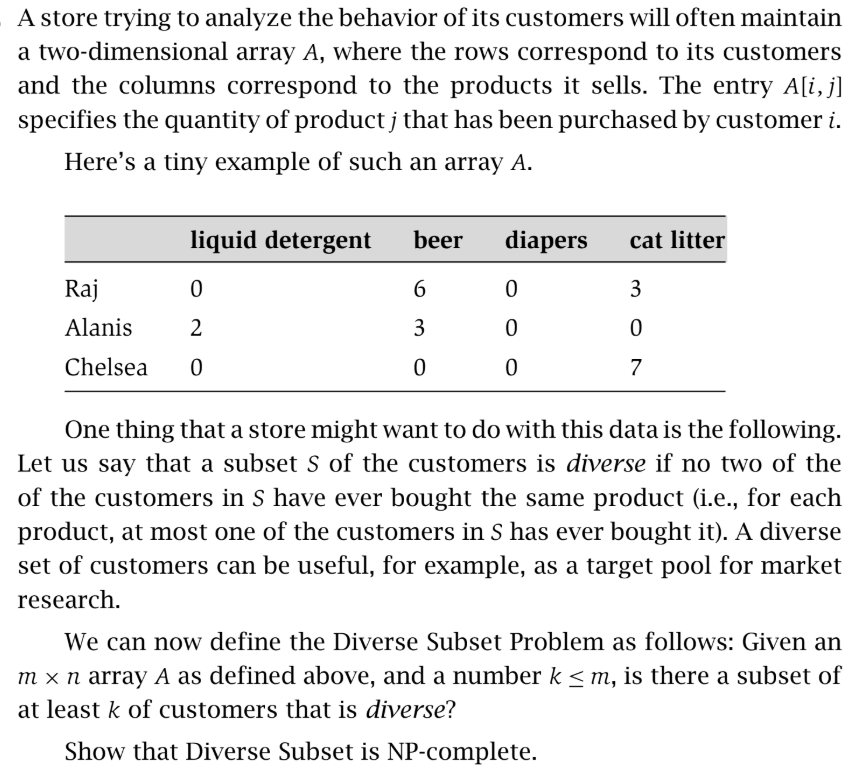
\includegraphics[scale=0.7]{images/q30.PNG}

We can make a reduction from Max Independent Set\\
Step 1: We construct a graph base on the purchase information recorded. We create a vertex for each customer. There is an edge between two customers if they bought a same product. This can be done in O(n) time, since the purchase information is already recorded \\

Step 2: If we can find a subset with the maximum set of vertices that doesn't share an edge in G, that means we can find a subset with the maximum number of customers that don't buy a same product. If k < max number, we output yes\\

Step 3: If we can find a subset of at least k customers that don't buy a same product, we can find a subset with the minimum number of vertices that doesn't share an edge in G. Then we can keep adding vertices to this minimum set to get a maximum. This can be done in O(V) time.  

\end{numedquestion}

\pagebreak
\begin{numedquestion}
Suppose you’re helping to organize a summer sports camp, and the following problem comes up. The camp is supposed to have at least one counselor who’s skilled at each of the n sports covered by the camp (baseball, volleyball, and so on). They have received job applications from m potential counselors. For each of the n sports, there is some subset of the m applicants qualified in that sport. The question is: For a given number k < m, is it possible to hire at most k of the counselors and have at least one counselor qualified in each of the n sports? We’ll call this the Efficient Recruiting Problem. Show that Efficient Recruiting is NP-complete.

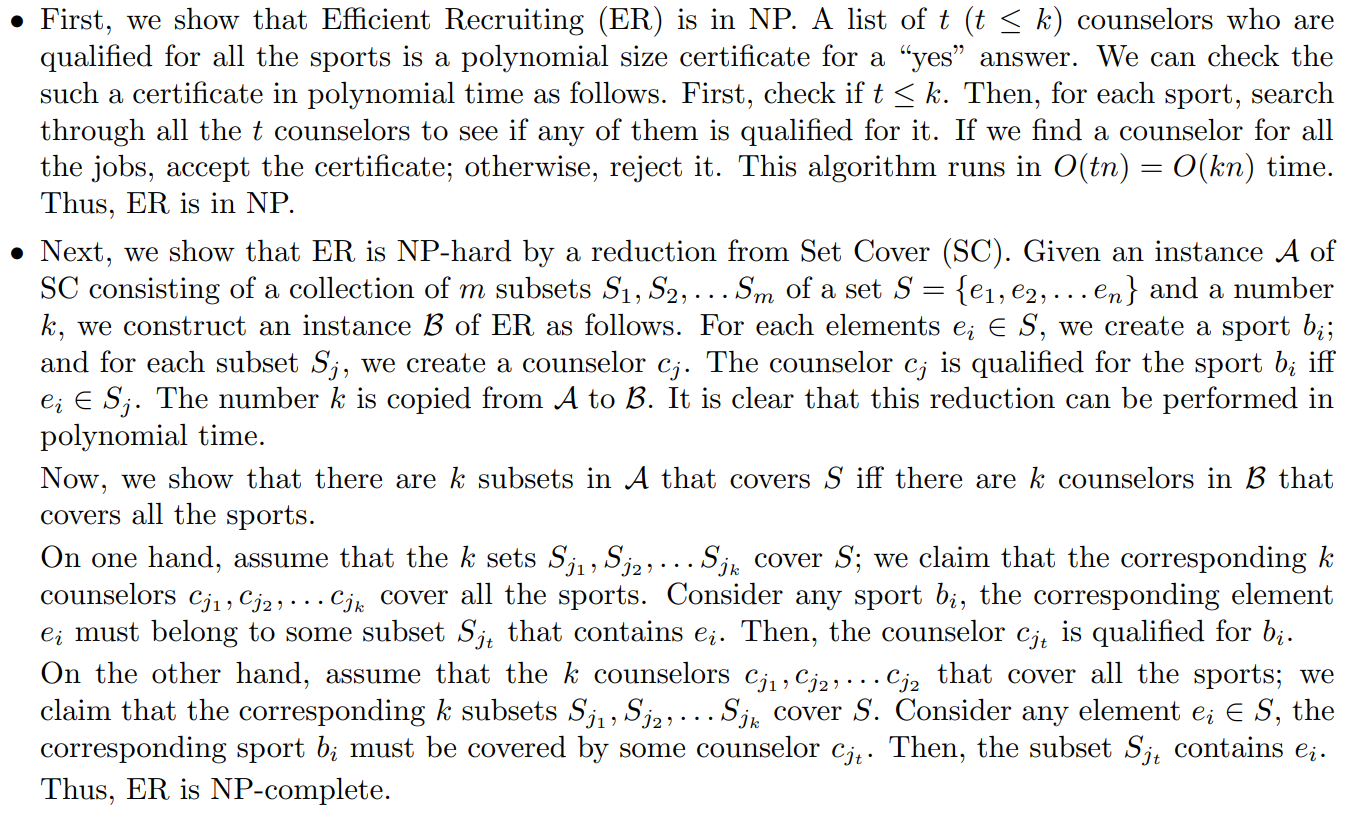
\includegraphics[scale=0.5]{images/q31sol.PNG}
\end{numedquestion}

\pagebreak
\begin{numedquestion}
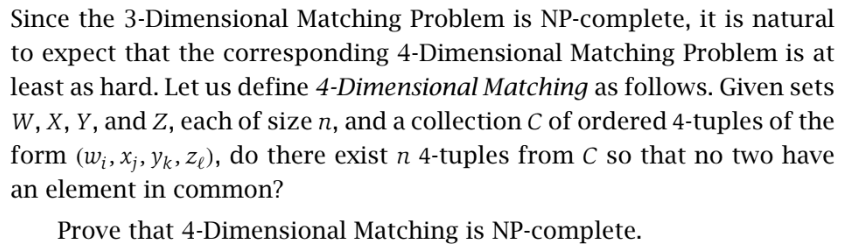
\includegraphics[scale=0.6]{images/q32.PNG} \\
We can make a reduction from 3D matching\\

Step 1: We can simply pad an extra coordinate to 3D by replicating the last coordinate, making the tuple (a,b,c,c)\\

Step 2: If we can find a 3D matching with (a,b,c), we can find a 4d matching (a,b,c,c), since c-c is simply a one-to-one correspondence\\ 

Step 3: If we can find a 4D matching with (a,b,c,c), we can find a 3d matching (a,b,c), since c-c is a one-to-one correspondence. 
\end{numedquestion}
\end{document}
